%%
%%
%% document.tex for  in /doctorat/ece/partenariat/cours/archi_kernel
%%
%% Made by Philippe THIERRY
%% Login   <Philippe THIERRYreseau-libre.net>
%%
%% Started on  Mon Sep  6 16:14:09 2010 Philippe THIERRY
%% Last update Wed Oct 13 17:24:03 2010 Philippe THIERRY
%%

%%%%%%%%%%%%%%%%%%%%%%%%%%%%%%%%%%%%%%%%%%%%%%%%%%%%%%%%%%%%%%%%%%%%%%%%%%%%%
%% Document style definition
%%%%%%%%%%%%%%%%%%%%%%%%%%%%%%%%%%%%%%%%%%%%%%%%%%%%%%%%%%%%%%%%%%%%%%%%%%%%%

\documentclass[twoside,a4paper,11pt,titlepage]{book} 	% document type


%%%%%%%%%%%%%%%%%%%%%%%%%%%%%%%%%%%%%%%%%%%%%%%%%%%%%%%%%%%%%%%%%%%%%%%%%%%%%
%% Packages integration
%%%%%%%%%%%%%%%%%%%%%%%%%%%%%%%%%%%%%%%%%%%%%%%%%%%%%%%%%%%%%%%%%%%%%%%%%%%%%

\usepackage[hundred]{vrsion}				% versioning support
\usepackage[latin1]{inputenc}				% char format
\usepackage{lscape}
\usepackage{rotating}
\usepackage[usenames,dvipsnames]{color}					% basic color support
\usepackage[T1]{fontenc} 				% caracteres norme iso-8859.
			 				% risque de ne pas marcher avec les fichiers crees
                         				% sous windows.
\usepackage[francais]{babel}			% french support
\usepackage{listings}					% lists support. Used for code
\usepackage{amsfonts}					% special fonts support (math, etc)
\usepackage{amsmath}
\usepackage{amssymb}					% special symbols support
\usepackage{graphicx}					% graphics integration support
\usepackage{fancyhdr}					% beautiful headers support
\usepackage{lastpage}					% \lastpage support
\usepackage{textcomp}					%
\usepackage[left=2.5cm,right=2.5cm,top=2.5cm,bottom=2.5cm]{geometry}
\usepackage{calc}					% counter support
\usepackage{datetime}					% personnalize dates
\usepackage{tabularx}					% tabular with more conf
\usepackage{array}					% tabular replacement
\usepackage{chngpage}					% change page layout localy
\usepackage{minitoc}
%
\usepackage{makeidx}
\usepackage[pdftex,
            pagebackref=true,
            colorlinks=true,
            linkcolor=blue
           ]{hyperref}					% allow interal links
           						% and doc content list 
\usepackage[all]{hypcap}
\usepackage{multirow}
\usepackage{multicol}
\usepackage{times}
\usepackage{ifpdf}
\usepackage{appendix} 
\usepackage{graphicx}
\usepackage{float}
\usepackage{alltt}
\usepackage[sectionbib]{natbib}
\usepackage{chapterbib}


\usepackage[Glenn]{fncychap}				% 'Glenn' chapter titles
\usepackage{supertabular}


% charts support
\usepackage{pdftricks}
\begin{psinputs}
  \usepackage{pstricks}
  \usepackage{multido}
  \usepackage{epsfig}
  \usepackage{pst-grad} % For gradients
  \usepackage{pst-plot} % For axes
  \usepackage{pst-tree} % For trees
  \usepackage{pst-3d} % For three dimensionnal graph
\end{psinputs}

%\usepackage{draftcopy}				% mark doc as 'draft'
%\draftcopyName{Provisoire}

%%%%%%%%%%%%%%%%%%%%%%%%%%%%%%%%%%%%%%%%%%%%%%%%%%%%%%%%%%%%%%%%%%%%%%%%%%%%%
%% Watermark for draft versions
%%%%%%%%%%%%%%%%%%%%%%%%%%%%%%%%%%%%%%%%%%%%%%%%%%%%%%%%%%%%%%%%%%%%%%%%%%%%%
\newcommand{\draftmode}{y}

\ifthenelse{\equal{\draftmode}{y}}{
  \usepackage{graphics,color} %
  \usepackage{eso-pic} % Required for Draft (\AddToShipoutPicture)
  \AddToShipoutPicture{\resizebox{0.7\pdfpagewidth}{0.7\pdfpageheight}%
  {\rotatebox{60}{\color[gray]{0.8}\hspace*{2.5cm}�BAUCHE}}}
}{}
%%%%%%%%%%%%%%%%%%%%%%%%%%%%%%%%%%%%%%%%%%%%%%%%%%%%%%%%%%%%%%%%%%%%%%%%%%%%%
%% Macro definition
%%%%%%%%%%%%%%%%%%%%%%%%%%%%%%%%%%%%%%%%%%%%%%%%%%%%%%%%%%%%%%%%%%%%%%%%%%%%%

%%%% Avoiding page orphalin %%%%
%%%% debut macro %%%%
\widowpenalty=10000
\clubpenalty=10000
\raggedbottom
%%%% fin macro %%%%

%%%% debut macro %%%%
\newenvironment{changemargin}[2]{\begin{list}{}{%	%
\addtolength{\leftmargin}{#1}%				% Support for local margin
\addtolength{\rightmargin}{#2}%				% update.
}\item }{\end{list}}					%
%%%% fin macro %%%%

% index support
\makeindex						% call for index generation


%\input{macros/myminitoc.sty}


% Add glossary
%\input{glossary.tex}

%%%%%%%%%%%%%%%%%%%%%%%%%%%%%%%%%%%%%%%%%%%%%%%%%%%%%%%%%%%%%%%%%%%%%%%%%%%%%
%% Code insertion support, using listing
%%%%%%%%%%%%%%%%%%%%%%%%%%%%%%%%%%%%%%%%%%%%%%%%%%%%%%%%%%%%%%%%%%%%%%%%%%%%%

% add code support
\definecolor{colKeys}{rgb}{0,0,1}			%
\definecolor{colIdentifier}{rgb}{0,0,0}			% Support for code coloration
\definecolor{colComments}{rgb}{0,0.5,1}			% Specify some colors
\definecolor{colString}{rgb}{0.6,0.1,0.1}		%

\lstset{%						% configuration of listings 
 float=hbp,% 						%
 basicstyle=\ttfamily\small, % 				% For code integration
 identifierstyle=\color{colIdentifier}, % 		% Use the above codekeys
 keywordstyle=\color{colKeys}, % 			% 
 stringstyle=\color{colString}, % 			%
 commentstyle=\color{colComments}, % 			%
 columns=flexible, % 					%
 tabsize=2, % 						%
 frame=trBL, % 						%
 frameround=tttt, % 					%
 extendedchars=true, % 					%
 showspaces=false, % 					%
 showstringspaces=false, % 				%
 numbers=left, % 					%
 numberstyle=\tiny, % 					%
 breaklines=true, % 					%
 breakautoindent=true, % 				%
 captionpos=b,% 					%
 xrightmargin=0.5cm, % 					%
     xleftmargin=0.5cm 					%
    } 							%

\lstloadlanguages{make,C}

\lstdefinelanguage{Make}
{
    keywords={ifeq,ifneq,ifdef,ifnded,else,endif,include},
    sensitive=true,
}


%%
%%
%% titlepage.tex for doctorat in /home/phil/Travail/Scolarité/Doctorat/doc/tex
%%
%% Made by Philippe THIERRY
%% Login   <Philippe THIERRYreseau-libre.net>
%%
%% Started on  mar. 24 nov. 2009 19:50:24 CET Philippe THIERRY
%% Last update Wed Oct 13 17:45:45 2010 Philippe THIERRY
%%

\newcommand{\thesisTitle}{
\changepage{3cm}{0cm}{0cm}{0cm}{0cm}{0cm}{-1cm}{0cm}{0cm}
\begin{center}
\begin{adjustwidth}{-1cm}{-1cm}
\begin{tabular}{p{9cm}p{8.5cm}}
\begin{flushleft}
\includegraphics[width=5cm]{pictures/ECE_LOGO_FR}\end{flushleft} &
%\begin{flushright}\includegraphics[width=5.5cm]{pictures/thales}\end{flushright} 
\\
\end{tabular}\\
\end{adjustwidth}
%\huge{\textbf{ECOLE CENTRALE D'ELECTRONIQUE\\
%PARIS}}\\
\vspace{1.1cm}
\large{\textsc{}}\\
\vspace{1.1cm}
Document �crit par\\
\vspace{0.5cm}
\Large{\textbf{Philippe THIERRY}}\\
\vspace{0.8cm}
dans le cadre des projets de l'ECE\\
\vspace{0.5cm}
\large{\textsc{}}\\
\vspace{1.8cm}
Sujet\\
\vspace{1.0cm}
\begin{adjustwidth}{-1cm}{-1cm}
\begin{tabular}[width=19cm]{||c||}
\hline
\hline
 \\
\huge{\textsc{Les architectures noyaux: un petit historique}}\\
\rule{3cm}{0.1ex}\\
\huge{\textsc{Introduction pour le d�veloppeur noyau Linux}}\\
\huge{\textsc{architecture et syst�me de production}}\\
  \\
\hline
\hline
\end{tabular}\\
\end{adjustwidth}
\vspace{2.5cm}
\small{\it version 0.5}\\
\vspace{1cm}
\normalsize{Avec la participation de}\\
\vspace{0.7cm}
\begin{tabular}{lll}
\large{Jean-Marc} & \large{LACROIX} & \large{jeanmarc.lacroix@free.fr} \\
\large{Sylvain} & \large{LEROY} & \large{sylvain@unmondelibre.fr} \\
\end{tabular}
\end{center}
\newpage
\changepage{-3cm}{0cm}{0cm}{0cm}{0cm}{0cm}{1cm}{0cm}{0cm}
}


% Set chaptername lowercase
\ChNameLowerCase
%%%%%%%%%%%%%%%%%%%%%%%%%%%%%%%%%%%%%%%%%%%%%%%%%%%%%%%%%%%%%%%%%%%%%%%%%%%%%
%% Headers and footers configuration
%%%%%%%%%%%%%%%%%%%%%%%%%%%%%%%%%%%%%%%%%%%%%%%%%%%%%%%%%%%%%%%%%%%%%%%%%%%%%

\pagestyle{fancy}					% specify page style
\pagenumbering{roman}					% specify page numbering
\fancyhf{}						% clear previous headers
%\addtolength{\headheight}{48pt}				% update header height


\newcommand{\FIXME}{\colorbox{yellow}{\textcolor{red}{FIXME}}}
%opening
\begin{document}

\selectlanguage{francais}

\dominitoc
\dominilot
\dominilof

\renewcommand{\headrulewidth}{0pt}			% disactive header bar


\fancyhead{}
\fancyfoot{}
\thesisTitle						% print title page
\fancyfoot[RO]{\thepage/\pageref{LastPage}}		% Right Odd foot
\fancyfoot[RE]{}					% Right Even foot
\fancyfoot[LE]{\thepage/\pageref{LastPage}}		% Left Even foot
\fancyfoot[LO]{}					% Left Odd foot

\cleardoublepage					% double blank page
\frontmatter						% out of TOC chapterss
\mainmatter						% starting TOC chapters

\cleardoublepage					% double blank page
%\dominitoc
\tableofcontents					% print table of contents
\listoffigures
\listoftables
\pagenumbering{arabic}					% update page number to arabic

\renewcommand{\headrulewidth}{1pt}			% allow header bar
\fancyhead[LO]{\leftmark}				% Left Odd header
\fancyhead[RE]{}					% Right Even header
\fancyhead[RO]{}					% Right Odd header
\fancyhead[LE]{\rightmark}				% Left Even header






%%%%%%%%%%%%%%%%%%%%%%%%%%%%%%%%%%%%%%%%%%%%%%%%%%%%%%%%%%%%%%%%%%%%%%%%%%%%%
%% Subfiles inclusion
%%%%%%%%%%%%%%%%%%%%%%%%%%%%%%%%%%%%%%%%%%%%%%%%%%%%%%%%%%%%%%%%%%%%%%%%%%%%%

%
% Seems to have a bug due to frontmatter/backmatter and the setcounter of
% chapter. To be fixed in the future.
%


%%
%%
%% introduction.tex for cours in /doctorat/ece/partenariat/cours/archi_kernel
%%
%% Made by Philippe THIERRY
%% Login   <Philippe THIERRYreseau-libre.net>
%%
%% Started on  Mon Sep  6 16:16:07 2010 Philippe THIERRY
%% Last update Mon Sep  6 16:16:27 2010 Philippe THIERRY
%%

\chapter{Introduction}


\paragraph{bar}


\part{Introductions aux architectures noyaux}

%%
%%
%% theo_kernel.tex for  in /doctorat/ece/partenariat/cours/archi_kernel
%%
%% Made by Philippe THIERRY
%% Login   <Philippe THIERRYreseau-libre.net>
%%
%% Started on  Wed Sep 22 14:45:23 2010 Philippe THIERRY
%% Last update Thu Sep 30 10:57:35 2010 Philippe THIERRY
%%

\chapter{Un petit historique du noyau}

\section{L'invention du noyau}

\section{Les noyaux monolithiques}

\paragraph{}
Historiquement le plus ancien, le noyau monolithique est la cons�quence des ajouts incessants de
nouvelles fonctionnalit�s dans les noyaux au fur et � mesure de l'int�gration de nouvelle
technologies.\\
En effet, les premiers noyaux ne poss�daient pas de pile r�seau et avait un nombre tr�s faible de
drivers. Avec la cr�ation du r�seau d'une part et l'h�t�rog�n�isation du mat�riel d'autre part,
beaucoup de code fut ajout� aux noyaux.

\begin{figure}[ht]
%%
%%
%% kernel_monolithic.tex for  in /doctorat/ece/partenariat/cours/archi_kernel
%%
%% Made by Philippe THIERRY
%% Login   <Philippe THIERRYreseau-libre.net>
%%
%% Started on  Thu Sep 23 14:19:58 2010 Philippe THIERRY
%% Last update Thu Sep 23 15:45:50 2010 Philippe THIERRY
%%

\begin{pdfpic}
\scalebox{1}{
\begin{pspicture}(0,0)(13,8)
% first line seems not to be considered by pstricks... strange...
\psline{-}(0,0)(0,0)
% kernel block
\definecolor{KernBase}{rgb}{0,0,0.7}
\definecolor{KernLow}{rgb}{0,0,0.6}
\psframe[linewidth=0.04cm,fillstyle=solid,fillcolor=KernBase](1,3)(11.5,0)
\psframe[linewidth=0.04cm,linestyle=dashed,fillstyle=solid,fillcolor=KernLow](1,1.6)(11.5,0)
\definecolor{UserBase}{rgb}{0.7,0.7,0.7}
\psframe[linewidth=0.0cm,fillstyle=solid,fillcolor=UserBase](1,3)(11.5,7.5)
%----- base kernel modules
\definecolor{KernModule}{rgb}{0,0,0.4}
\definecolor{KernShadow}{rgb}{0,0,0.1}
% memory module
\psframe[linewidth=0.00cm,fillstyle=solid,fillcolor=KernShadow,framearc=.3](1.6,0.4)(3.6,1.4) % shadow
\psframe[linewidth=0.04cm,fillstyle=solid,fillcolor=KernModule,framearc=.3](1.5,0.5)(3.5,1.5)
\rput(2.5,1){\text \color{white}{memory}}
% IRQ module
\psframe[linewidth=0.00cm,fillstyle=solid,fillcolor=KernShadow,framearc=.3](4.1,0.4)(6.1,1.4) % shadow
\psframe[linewidth=0.04cm,fillstyle=solid,fillcolor=KernModule,framearc=.3](4,0.5)(6,1.5)
\rput(5,1){\text \color{white}{interrupt}}
% sched module
\psframe[linewidth=0.00cm,fillstyle=solid,fillcolor=KernShadow,framearc=.3](6.6,0.4)(8.6,1.4) % shadow
\psframe[linewidth=0.04cm,fillstyle=solid,fillcolor=KernModule,framearc=.3](6.5,0.5)(8.5,1.5)
\rput(7.5,1){\text \color{white}{scheduler}}
% CPU module
\psframe[linewidth=0.00cm,fillstyle=solid,fillcolor=KernShadow,framearc=.3](9.1,0.4)(11.1,1.4) % shadow
\psframe[linewidth=0.04cm,fillstyle=solid,fillcolor=KernModule,framearc=.3](9,0.5)(11,1.5)
\rput(10,1){\text \color{white}{processor}}
%----- high kernel modules
\definecolor{KernModule2}{rgb}{0.3,0,0.3}
\definecolor{KernShadow2}{rgb}{0.1,0,0.1}
% driver modules
\psframe[linewidth=0.00cm,fillstyle=solid,fillcolor=KernShadow2,framearc=.3](1.6,1.7)(3.6,2.7) % shadow
\psframe[linewidth=0.04cm,fillstyle=solid,fillcolor=KernModule2,framearc=.3](1.5,1.8)(3.5,2.8)
\rput(2.5,2.3){\text \color{white}{drivers}}
% network module
\psframe[linewidth=0.00cm,fillstyle=solid,fillcolor=KernShadow2,framearc=.3](4.1,1.7)(6.1,2.7) % shadow
\psframe[linewidth=0.04cm,fillstyle=solid,fillcolor=KernModule2,framearc=.3](4,1.8)(6,2.8)
\rput(5,2.3){\text \color{white}{network}}
% fs module
\psframe[linewidth=0.00cm,fillstyle=solid,fillcolor=KernShadow2,framearc=.3](6.6,1.7)(8.6,2.7) % shadow
\psframe[linewidth=0.04cm,fillstyle=solid,fillcolor=KernModule2,framearc=.3](6.5,1.8)(8.5,2.8)
\rput(7.5,2.3){\text \color{white}{filesystem}}
% syscall, IPC module
\psframe[linewidth=0.00cm,fillstyle=solid,fillcolor=KernShadow2,framearc=.3](9.1,1.7)(11.1,2.7) % shadow
\psframe[linewidth=0.04cm,fillstyle=solid,fillcolor=KernModule2,framearc=.3](9,1.8)(11,2.8)
\rput(10,2.3){\text \color{white}{syscalls}}
% US/KS separation line
\psline[linewidth=0.05cm,linestyle=dashed]{-}(0.5,3)(12,3)
\rput{90}(12,1.5){\text kernelspace}
%--- library
\definecolor{Library}{rgb}{0,0.3,0}
\definecolor{LibraryShadow}{rgb}{0,0.1,0}
% lib 1
\psframe[linewidth=0.00cm,fillstyle=solid,fillcolor=LibraryShadow,framearc=.3](1.3,3.1)(4.3,3.9)
\psframe[linewidth=0.04cm,fillstyle=solid,fillcolor=Library,framearc=.3](1.2,3.2)(4.2,4)
\rput(2.7,3.6){\text \color{white}{Library}}
% lib 2
\psframe[linewidth=0.00cm,fillstyle=solid,fillcolor=LibraryShadow,framearc=.3](4.6,3.1)(7.6,3.9)
\psframe[linewidth=0.04cm,fillstyle=solid,fillcolor=Library,framearc=.3](4.5,3.2)(7.5,4)
\rput(6.1,3.6){\text \color{white}{Library}}
% lib 3
\psframe[linewidth=0.00cm,fillstyle=solid,fillcolor=LibraryShadow,framearc=.3](7.9,3.1)(10.9,3.9)
\psframe[linewidth=0.04cm,fillstyle=solid,fillcolor=Library,framearc=.3](7.8,3.2)(10.8,4)
\rput(9.4,3.6){\text \color{white}{Library}}
%--- tasks
\definecolor{Task}{rgb}{0.3,0,0}
\definecolor{TaskShadow}{rgb}{0.1,0,0}
% first task
\psframe[linewidth=0.0cm,fillstyle=solid,fillcolor=TaskShadow,framearc=.3](1.6,4.1)(3.1,7.1)
\psframe[linewidth=0.04cm,fillstyle=solid,fillcolor=Task,framearc=.3](1.5,4.2)(3,7.2)
\rput{60}(2.25,5.7){\text \color{white}{first task}}
% second task
\psframe[linewidth=0.0cm,fillstyle=solid,fillcolor=TaskShadow,framearc=.3](3.6,4.1)(5.1,7.1)
\psframe[linewidth=0.04cm,fillstyle=solid,fillcolor=Task,framearc=.3](3.5,4.2)(5,7.2)
\rput{60}(4.25,5.7){\text \color{white}{second task}}
% etc line
\psline[linewidth=0.04cm,linestyle=dotted](5.4,5.7)(6.6,5.7)
% third task
\psframe[linewidth=0.0cm,fillstyle=solid,fillcolor=TaskShadow,framearc=.3](7.1,4.1)(8.6,7.1)
\psframe[linewidth=0.04cm,fillstyle=solid,fillcolor=Task,framearc=.3](7,4.2)(8.5,7.2)
\rput{60}(7.75,5.7){\text \color{white}{{\it N-1}\textsuperscript{th} task}}
% fourth task
\psframe[linewidth=0.0cm,fillstyle=solid,fillcolor=TaskShadow,framearc=.3](9.1,4.1)(10.6,7.1)
\psframe[linewidth=0.04cm,fillstyle=solid,fillcolor=Task,framearc=.3](9,4.2)(10.5,7.2)
\rput{60}(9.75,5.7){\text \color{white}{{\it N}\textsuperscript{th} task}}
\rput{90}(12,5.25){\text userspace}
\rput{90}(0.6,0.75){\text bases}
\rput{90}(0.6,2.25){\text add-ons}
\end{pspicture}
}
\end{pdfpic}

\label{pic:kern_monolithic}
\caption{R�partition des services dans un noyau monolithique}
\end{figure}

\section{Les noyaux hybrides}

\paragraph{}
Exemple de GNU Hurd, noyau hybride �crit en C++, d�portant une partie de ses modules dans un
domaine d'ex�cution dit de {\it service}, hors de l'espace d'adressage du noyau. Un plantage dans
cette zone de service ne provoque pas de plantage du noyau, du fait de cette s�paration.

\begin{figure}[ht]
%%
%%
%% kernel_monolithic.tex for  in /doctorat/ece/partenariat/cours/archi_kernel
%%
%% Made by Philippe THIERRY
%% Login   <Philippe THIERRYreseau-libre.net>
%%
%% Started on  Thu Sep 23 14:19:58 2010 Philippe THIERRY
%% Last update Thu Sep 23 16:50:25 2010 Philippe THIERRY
%%

\begin{pdfpic}
\scalebox{1}{
\begin{pspicture}(0,0)(13,8)
% first line seems not to be considered by pstricks... strange...
\psline{-}(0,0)(0,0)
% kernel block
\definecolor{Service}{rgb}{0.81,0.73,0.20}
\definecolor{KernLow}{rgb}{0,0,0.6}
\psframe[linewidth=0.04cm,fillstyle=solid,fillcolor=Service](1,3)(11.5,1.5)
\psframe[linewidth=0.04cm,linestyle=dashed,fillstyle=solid,fillcolor=KernLow](1,1.6)(11.5,0)
\definecolor{UserBase}{rgb}{0.7,0.7,0.7}
\psframe[linewidth=0.0cm,fillstyle=solid,fillcolor=UserBase](1,3)(11.5,7.5)
%----- base kernel modules
\definecolor{KernModule}{rgb}{0,0,0.4}
\definecolor{KernShadow}{rgb}{0,0,0.1}
% memory module
\psframe[linewidth=0.00cm,fillstyle=solid,fillcolor=KernShadow,framearc=.3](1.6,0.4)(3.6,1.4) % shadow
\psframe[linewidth=0.04cm,fillstyle=solid,fillcolor=KernModule,framearc=.3](1.5,0.5)(3.5,1.5)
\rput(2.5,1){\text \color{white}{memory}}
% IRQ module
\psframe[linewidth=0.00cm,fillstyle=solid,fillcolor=KernShadow,framearc=.3](4.1,0.4)(6.1,1.4) % shadow
\psframe[linewidth=0.04cm,fillstyle=solid,fillcolor=KernModule,framearc=.3](4,0.5)(6,1.5)
\rput(5,1){\text \color{white}{interrupt}}
% sched module
\psframe[linewidth=0.00cm,fillstyle=solid,fillcolor=KernShadow,framearc=.3](6.6,0.4)(8.6,1.4) % shadow
\psframe[linewidth=0.04cm,fillstyle=solid,fillcolor=KernModule,framearc=.3](6.5,0.5)(8.5,1.5)
\rput(7.5,1){\text \color{white}{scheduler}}
% CPU module
\psframe[linewidth=0.00cm,fillstyle=solid,fillcolor=KernShadow,framearc=.3](9.1,0.4)(11.1,1.4) % shadow
\psframe[linewidth=0.04cm,fillstyle=solid,fillcolor=KernModule,framearc=.3](9,0.5)(11,1.5)
\rput(10,1){\text \color{white}{processor}}
%----- high kernel modules
\definecolor{ServiceModule}{rgb}{0.405,0.365,0.10}
\definecolor{ServiceShadow}{rgb}{0.202,0.18,0.05}
% driver modules
\psframe[linewidth=0.00cm,fillstyle=solid,fillcolor=ServiceShadow,framearc=.3](1.6,1.7)(3.6,2.7) % shadow
\psframe[linewidth=0.04cm,fillstyle=solid,fillcolor=ServiceModule,framearc=.3](1.5,1.8)(3.5,2.8)
\rput(2.5,2.3){\text \color{white}{drivers}}
% network module
\psframe[linewidth=0.00cm,fillstyle=solid,fillcolor=ServiceShadow,framearc=.3](4.1,1.7)(6.1,2.7) % shadow
\psframe[linewidth=0.04cm,fillstyle=solid,fillcolor=ServiceModule,framearc=.3](4,1.8)(6,2.8)
\rput(5,2.3){\text \color{white}{network}}
% fs module
\psframe[linewidth=0.00cm,fillstyle=solid,fillcolor=ServiceShadow,framearc=.3](6.6,1.7)(8.6,2.7) % shadow
\psframe[linewidth=0.04cm,fillstyle=solid,fillcolor=ServiceModule,framearc=.3](6.5,1.8)(8.5,2.8)
\rput(7.5,2.3){\text \color{white}{filesystem}}
% syscall, IPC module
\psframe[linewidth=0.00cm,fillstyle=solid,fillcolor=ServiceShadow,framearc=.3](9.1,1.7)(11.1,2.7) % shadow
\psframe[linewidth=0.04cm,fillstyle=solid,fillcolor=ServiceModule,framearc=.3](9,1.8)(11,2.8)
\rput(10,2.3){\text \color{white}{syscalls}}
% US/KS separation line
\psline[linewidth=0.05cm,linestyle=dashed]{-}(0.5,1.6)(12,1.6)
\rput{90}(12,0.75){\text {\small kernelspace}}
%--- library
\definecolor{Library}{rgb}{0,0.3,0}
\definecolor{LibraryShadow}{rgb}{0,0.1,0}
% lib 1
\psframe[linewidth=0.00cm,fillstyle=solid,fillcolor=LibraryShadow,framearc=.3](1.3,3.1)(4.3,3.9)
\psframe[linewidth=0.04cm,fillstyle=solid,fillcolor=Library,framearc=.3](1.2,3.2)(4.2,4)
\rput(2.7,3.6){\text \color{white}{Library}}
% lib 2
\psframe[linewidth=0.00cm,fillstyle=solid,fillcolor=LibraryShadow,framearc=.3](4.6,3.1)(7.6,3.9)
\psframe[linewidth=0.04cm,fillstyle=solid,fillcolor=Library,framearc=.3](4.5,3.2)(7.5,4)
\rput(6.1,3.6){\text \color{white}{Library}}
% lib 3
\psframe[linewidth=0.00cm,fillstyle=solid,fillcolor=LibraryShadow,framearc=.3](7.9,3.1)(10.9,3.9)
\psframe[linewidth=0.04cm,fillstyle=solid,fillcolor=Library,framearc=.3](7.8,3.2)(10.8,4)
\rput(9.4,3.6){\text \color{white}{Library}}
%--- tasks
\definecolor{Task}{rgb}{0.3,0,0}
\definecolor{TaskShadow}{rgb}{0.1,0,0}
% first task
\psframe[linewidth=0.0cm,fillstyle=solid,fillcolor=TaskShadow,framearc=.3](1.6,4.1)(3.1,7.1)
\psframe[linewidth=0.04cm,fillstyle=solid,fillcolor=Task,framearc=.3](1.5,4.2)(3,7.2)
\rput{60}(2.25,5.7){\text \color{white}{first task}}
% second task
\psframe[linewidth=0.0cm,fillstyle=solid,fillcolor=TaskShadow,framearc=.3](3.6,4.1)(5.1,7.1)
\psframe[linewidth=0.04cm,fillstyle=solid,fillcolor=Task,framearc=.3](3.5,4.2)(5,7.2)
\rput{60}(4.25,5.7){\text \color{white}{second task}}
% etc line
\psline[linewidth=0.04cm,linestyle=dotted](5.4,5.7)(6.6,5.7)
% third task
\psframe[linewidth=0.0cm,fillstyle=solid,fillcolor=TaskShadow,framearc=.3](7.1,4.1)(8.6,7.1)
\psframe[linewidth=0.04cm,fillstyle=solid,fillcolor=Task,framearc=.3](7,4.2)(8.5,7.2)
\rput{60}(7.75,5.7){\text \color{white}{{\it N-1}\textsuperscript{th} task}}
% fourth task
\psframe[linewidth=0.0cm,fillstyle=solid,fillcolor=TaskShadow,framearc=.3](9.1,4.1)(10.6,7.1)
\psframe[linewidth=0.04cm,fillstyle=solid,fillcolor=Task,framearc=.3](9,4.2)(10.5,7.2)
\rput{60}(9.75,5.7){\text \color{white}{{\it N}\textsuperscript{th} task}}
\rput{90}(12,5.25){\text userspace}
\rput{90}(0.6,0.75){\text base}
% service/userspace line
\psline[linewidth=0.05cm,linestyle=dashed]{-}(0.5,3)(12,3)
\rput{90}(0.6,2.25){\text services}
\end{pspicture}
}
\end{pdfpic}

\label{pic:kern_hybrid}
\caption{R�partition des services dans un noyau hybride}
\end{figure}


\section{Les micro-noyaux}

\begin{figure}[ht]
%%
%%
%% kernel_monolithic.tex for  in /doctorat/ece/partenariat/cours/archi_kernel
%%
%% Made by Philippe THIERRY
%% Login   <Philippe THIERRYreseau-libre.net>
%%
%% Started on  Thu Sep 23 14:19:58 2010 Philippe THIERRY
%% Last update Wed Sep 29 14:35:36 2010 Philippe THIERRY
%%

\begin{pdfpic}
\scalebox{0.8}{
\begin{pspicture}(0,0)(15,8)
% first line seems not to be considered by pstricks... strange...
\psline{-}(0,0)(0,0)
% kernel block
\definecolor{KernLow}{rgb}{0,0,0.6}
\psframe[linewidth=0.04cm,linestyle=dashed,fillstyle=solid,fillcolor=KernLow](1,1.8)(14,0)
\definecolor{UserBase}{rgb}{0.7,0.7,0.7}
% background of userspace content
\psframe[linewidth=0.0cm,fillstyle=solid,fillcolor=UserBase](1,1.8)(14,5.5)
%----- base kernel modules
\definecolor{KernModule}{rgb}{0,0,0.4}
\definecolor{KernShadow}{rgb}{0,0,0.1}
% memory module
\psframe[linewidth=0.00cm,fillstyle=solid,fillcolor=KernShadow,framearc=.3](1.6,0.4)(3.6,1.4) % shadow
\psframe[linewidth=0.04cm,fillstyle=solid,fillcolor=KernModule,framearc=.3](1.5,0.5)(3.5,1.5)
\rput(2.5,1){\text \color{white}{memory}}
% IRQ module
\psframe[linewidth=0.00cm,fillstyle=solid,fillcolor=KernShadow,framearc=.3](4.1,0.4)(6.1,1.4) % shadow
\psframe[linewidth=0.04cm,fillstyle=solid,fillcolor=KernModule,framearc=.3](4,0.5)(6,1.5)
\rput(5,1){\text \color{white}{interrupt}}
% sched module
\psframe[linewidth=0.00cm,fillstyle=solid,fillcolor=KernShadow,framearc=.3](6.6,0.4)(8.6,1.4) % shadow
\psframe[linewidth=0.04cm,fillstyle=solid,fillcolor=KernModule,framearc=.3](6.5,0.5)(8.5,1.5)
\rput(7.5,1){\text \color{white}{scheduler}}
% CPU module
\psframe[linewidth=0.00cm,fillstyle=solid,fillcolor=KernShadow,framearc=.3](9.1,0.4)(11.1,1.4) % shadow
\psframe[linewidth=0.04cm,fillstyle=solid,fillcolor=KernModule,framearc=.3](9,0.5)(11,1.5)
\rput(10,1){\text \color{white}{processor}}
% IPC module
\psframe[linewidth=0.00cm,fillstyle=solid,fillcolor=KernShadow,framearc=.3](11.6,0.4)(13.6,1.4) % shadow
\psframe[linewidth=0.04cm,fillstyle=solid,fillcolor=KernModule,framearc=.3](11.5,0.5)(13.5,1.5)
\rput(12.5,1){\text \color{white}{IPC}}
% service/userspace line
\psline[linewidth=0.05cm,linestyle=dashed]{-}(0.5,1.8)(14.5,1.8)
%--- tasks
\definecolor{Library}{rgb}{0,0.3,0}
\definecolor{LibraryShadow}{rgb}{0,0.1,0}
\definecolor{Task}{rgb}{0.3,0,0}
\definecolor{TaskShadow}{rgb}{0.1,0,0}
% first task
\psframe[linewidth=0.0cm,fillstyle=solid,fillcolor=TaskShadow,framearc=.3](1.6,2.1)(3.1,5.1)
\psframe[linewidth=0.04cm,fillstyle=solid,fillcolor=Task,framearc=.3](1.5,2.2)(3,5.2)
\rput{60}(2.25,3.7){\text \color{white}{first task}}
% second task
\psframe[linewidth=0.0cm,fillstyle=solid,fillcolor=TaskShadow,framearc=.3](3.6,2.1)(5.1,5.1)
\psframe[linewidth=0.04cm,fillstyle=solid,fillcolor=Task,framearc=.3](3.5,2.2)(5,5.2)
\rput{60}(4.25,3.7){\text \color{white}{second task}}
% library
\psframe[linewidth=0.0cm,fillstyle=solid,fillcolor=LibraryShadow,framearc=.3](5.6,2.1)(7.1,5.1)
\psframe[linewidth=0.04cm,fillstyle=solid,fillcolor=Library,framearc=.3](5.5,2.2)(7,5.2)
\rput{60}(6.25,3.7){\text \color{white}{service}}
% third task
\psframe[linewidth=0.0cm,fillstyle=solid,fillcolor=TaskShadow,framearc=.3](7.6,2.1)(9.1,5.1)
\psframe[linewidth=0.04cm,fillstyle=solid,fillcolor=Task,framearc=.3](7.5,2.2)(9,5.2)
\rput{60}(8.25,3.7){\text \color{white}{{\it N-1}\textsuperscript{th} task}}
% fourth task
\definecolor{Driver}{rgb}{0.405,0.365,0.10}
\definecolor{DriverShadow}{rgb}{0.202,0.18,0.05}
\psframe[linewidth=0.0cm,fillstyle=solid,fillcolor=TaskShadow,framearc=.3](9.6,2.1)(11.1,5.1)
\psframe[linewidth=0.04cm,fillstyle=solid,fillcolor=Task,framearc=.3](9.5,2.2)(11,5.2)
\rput{60}(10.25,3.7){\text \color{white}{{\it N}\textsuperscript{th} task}}
% driver
\definecolor{Driver}{rgb}{0.405,0.365,0.10}
\definecolor{DriverShadow}{rgb}{0.202,0.18,0.05}
\definecolor{Task}{rgb}{0.3,0,0}
\psframe[linewidth=0.0cm,fillstyle=solid,fillcolor=DriverShadow,framearc=.3](11.6,2.1)(13.1,5.1)
\psframe[linewidth=0.04cm,fillstyle=solid,fillcolor=Driver,framearc=.3](11.5,2.2)(13,5.2)
\rput{60}(12.25,3.7){\text \color{white}{driver}}
% other legends
\rput{90}(14.5,3.7){\text userspace}
\rput{90}(14.5,0.75){\text kernelpace}
\rput{90}(0.6,0.75){\text $\mu$-kernel}
\end{pspicture}
}
\end{pdfpic}

\label{pic:kern_micro}
\caption{Les architectures � base de micro-noyaux}
\end{figure}


\section{Les noyaux d'aujourd'hui}

\subsection{Les exo-noyaux}

\paragraph{}
Il existe aujourd'hui des �l�ments d'architectures de type exo-noyaux. Il s'agit de noyau plus
petits encore que les micro-noyaux d�crits au dessus. Le but est de fournir uniquement une couche
d'abstraction du mat�riel sans fournir d'�l�ments avanc�s tels qu'un ordonnanceur au niveau noyau.

\paragraph{}
Les exo-noyaux sont destin�s � des architectures logicielles peu fr�quentes (\FIXME continuer)

\subsection{Les hyperviseurs}

\paragraph{}
Bien que le principe de virtualisation date de 1973, son v�ritable essor date du d�but des ann�es
2000, pour des raisons diverses :
\begin{itemize}
\item La puissance des machines, suffisante pour fournir plusieurs services simultan�ment 
\item La r�duction du co�t du mat�riel et de la consommation �lectrique
\item Un besoin de redondance logicielle, simple � g�rer via la virtualisation
\item La possibilit� de maqu�ter rapidement et efficacement des architectures r�seaux complexes
\item Plus r�cemment un besoin de s�curit� au travers du cloisonnement par la virtualisation. Ce
dernier �l�ment est moins connu du grand public et s'appuie sur des solutions autres que les
c�l�bres VMWare et VirtualBox.
\end{itemize}

\paragraph{}
Parmis les diff�rentes solutions de virtualisation, il existe les hyperviseurs, solutions bas�es
sur un noyau plus ou moins gros, dont l'acc�s n'est jamais direct. On passe alors par des consoles
de gestion (cas de certains hyperviseurs professionnels) ou des domaines virtuels dits "privil�gi�s"
(cas de Xen). Ces hyperviseurs fournissent des services de type paravirtualisation ou de type HVM
(Hardware-based Virtual-machine Monitor, s'appuyant sur des composants mat�riels tels que Intel VT
ou ARM TrustZone).

\begin{figure}[ht]
%%
%%
%% kernel_monolithic.tex for  in /doctorat/ece/partenariat/cours/archi_kernel
%%
%% Made by Philippe THIERRY
%% Login   <Philippe THIERRYreseau-libre.net>
%%
%% Started on  Thu Sep 23 14:19:58 2010 Philippe THIERRY
%% Last update Wed Sep 29 15:25:02 2010 Philippe THIERRY
%%

\begin{pdfpic}
\scalebox{0.8}{
\begin{pspicture}(0,0)(15,8)
% first line seems not to be considered by pstricks... strange...
\psline{-}(0,0)(0,0)
% kernel block
\definecolor{KernLow}{rgb}{0,0,0.6}
\psframe[linewidth=0.04cm,linestyle=dashed,fillstyle=solid,fillcolor=KernLow](1,1.8)(14,0)
\definecolor{UserBase}{rgb}{0.7,0.7,0.7}
% background of userspace content
\psframe[linewidth=0.0cm,fillstyle=solid,fillcolor=UserBase](1,1.8)(14,7.5)
%----- base kernel modules
\definecolor{KernModule}{rgb}{0,0,0.4}
\definecolor{KernShadow}{rgb}{0,0,0.1}
% memory module
\psframe[linewidth=0.00cm,fillstyle=solid,fillcolor=KernShadow,framearc=.3](1.6,0.4)(3.6,1.4) % shadow
\psframe[linewidth=0.04cm,fillstyle=solid,fillcolor=KernModule,framearc=.3](1.5,0.5)(3.5,1.5)
\rput(2.5,1){\text \color{white}{memory}}
% IRQ module
\psframe[linewidth=0.00cm,fillstyle=solid,fillcolor=KernShadow,framearc=.3](4.1,0.4)(6.1,1.4) % shadow
\psframe[linewidth=0.04cm,fillstyle=solid,fillcolor=KernModule,framearc=.3](4,0.5)(6,1.5)
\rput(5,1){\text \color{white}{interrupt}}
% sched module
\psframe[linewidth=0.00cm,fillstyle=solid,fillcolor=KernShadow,framearc=.3](6.6,0.4)(8.6,1.4) % shadow
\psframe[linewidth=0.04cm,fillstyle=solid,fillcolor=KernModule,framearc=.3](6.5,0.5)(8.5,1.5)
\rput(7.5,1){\text \color{white}{scheduler}}
% CPU module
\psframe[linewidth=0.00cm,fillstyle=solid,fillcolor=KernShadow,framearc=.3](9.1,0.4)(11.1,1.4) % shadow
\psframe[linewidth=0.04cm,fillstyle=solid,fillcolor=KernModule,framearc=.3](9,0.5)(11,1.5)
\rput(10,1){\text \color{white}{processor}}
% IPC module
\psframe[linewidth=0.00cm,fillstyle=solid,fillcolor=KernShadow,framearc=.3](11.6,0.4)(13.6,1.4) % shadow
\psframe[linewidth=0.04cm,fillstyle=solid,fillcolor=KernModule,framearc=.3](11.5,0.5)(13.5,1.5)
\rput(12.5,1){\text \color{white}{IPC}}
% service/userspace line
\psline[linewidth=0.05cm,linestyle=dashed]{-}(0.5,1.8)(15,1.8)
% Native hypervision interface
\definecolor{Library}{rgb}{0,0.3,0}
\psframe[linewidth=0.04cm,fillstyle=solid,fillcolor=Library,framearc=.3](1,1.8)(14,2.5)
\rput(7.5,2.1){\text native hypervision interface}
%--- tasks
\definecolor{LibraryShadow}{rgb}{0,0.1,0}
\definecolor{Task}{rgb}{0.3,0,0}
\definecolor{TaskShadow}{rgb}{0.1,0,0}
% first task
\psframe[linewidth=0.0cm,fillstyle=solid,fillcolor=TaskShadow,framearc=.3](1.6,2.7)(3.1,7.1)
\psframe[linewidth=0.04cm,fillstyle=solid,fillcolor=Task,framearc=.3](1.5,2.8)(3,7.2)
\rput{60}(2.25,5){\text \color{white}{first native task}}
% second task
\psframe[linewidth=0.0cm,fillstyle=solid,fillcolor=TaskShadow,framearc=.3](3.6,2.7)(5.1,7.1)
\psframe[linewidth=0.04cm,fillstyle=solid,fillcolor=Task,framearc=.3](3.5,2.8)(5,7.2)
\rput{60}(4.25,5){\text \color{white}{second native task}}

% OS
\definecolor{OSColor}{rgb}{0.2,0.2,0.2}
\definecolor{OSColorShadow}{rgb}{0.1,0.1,0.1}
% guest OS bg
\psframe[linewidth=0.04cm,fillstyle=solid,fillcolor=OSColorShadow,framearc=0.3](5.6,2.7)(7.1,7.1)
\psframe[linewidth=0.04cm,fillstyle=solid,fillcolor=OSColor,framearc=0.3](5.5,2.8)(7,7.2)
% guest OS virtualized kernel
\psframe[linewidth=0.0cm,fillstyle=solid,fillcolor=KernLow,linecolor=black,framearc=.3](5.5,2.8)(7,4)
\rput(6.25,3.3){\text \color{white}{kernel}}
% guest OS lib
\psframe[linewidth=0.04cm,fillstyle=solid,fillcolor=Library,framearc=.3](5.5,4.1)(7,5.1)
\rput(6.25,4.5){\text \color{white}{library}}
% guest OS tasks
\psframe[linewidth=0.04cm,fillstyle=solid,fillcolor=Task](5.6,5.1)(5.9,7)
\psframe[linewidth=0.04cm,fillstyle=solid,fillcolor=Task](6,5.1)(6.3,7)
\psframe[linewidth=0.04cm,fillstyle=solid,fillcolor=Task](6.4,5.1)(6.7,7)

% OS
\definecolor{OSColor}{rgb}{0.2,0.2,0.2}
\definecolor{OSColorShadow}{rgb}{0.1,0.1,0.1}
% guest OS bg
\psframe[linewidth=0.04cm,fillstyle=solid,fillcolor=OSColorShadow,framearc=0.3](7.6,2.7)(9.1,7.1)
\psframe[linewidth=0.04cm,fillstyle=solid,fillcolor=OSColor,framearc=0.3](7.5,2.8)(9,7.2)
% guest OS virtualized kernel
\psframe[linewidth=0.0cm,fillstyle=solid,fillcolor=KernLow,linecolor=black,framearc=.3](7.5,2.8)(9,4)
\rput(8.25,3.3){\text \color{white}{kernel}}
% guest OS lib
\psframe[linewidth=0.04cm,fillstyle=solid,fillcolor=Library,framearc=.3](7.5,4.1)(9,5.1)
\rput(8.25,4.5){\text \color{white}{library}}
% guest OS tasks
\psframe[linewidth=0.04cm,fillstyle=solid,fillcolor=Task](7.6,5.1)(7.9,7)
\psframe[linewidth=0.04cm,fillstyle=solid,fillcolor=Task](8,5.1)(8.3,7)
\psframe[linewidth=0.04cm,fillstyle=solid,fillcolor=Task](8.4,5.1)(8.7,7)

% fourth task
\definecolor{Driver}{rgb}{0.405,0.365,0.10}
\definecolor{DriverShadow}{rgb}{0.202,0.18,0.05}
\psframe[linewidth=0.0cm,fillstyle=solid,fillcolor=TaskShadow,framearc=.3](9.6,2.7)(11.1,7.1)
\psframe[linewidth=0.04cm,fillstyle=solid,fillcolor=Task,framearc=.3](9.5,2.8)(11,7.2)
\rput{60}(10.25,5){\text \color{white}{third native task}}
% driver
\definecolor{Task}{rgb}{0.3,0,0}
\psframe[linewidth=0.0cm,fillstyle=solid,fillcolor=DriverShadow,framearc=.3](11.6,2.7)(13.1,7.1)
\psframe[linewidth=0.04cm,fillstyle=solid,fillcolor=Driver,framearc=.3](11.5,2.8)(13,7.2)
\rput{60}(12.25,5){\text \color{white}{driver}}
% other legends
\rput{90}(14.5,5.25){\text userspace}
\rput{90}(14.5,0.75){\text kernelspace}
\rput{90}(0.6,0.75){\text hypervisor}
\end{pspicture}
}
\end{pdfpic}

\label{pic:kern_micro}
\caption{Les architectures logiciels des hyperviseurs}
\end{figure}

\paragraph{}
Les hyperviseurs permettent de supporter des machines virtuelles avec un choix plus ou moins riche
et un cloisonnement plus ou moins fort\footnote{Pour ceux que �a int�resse, il est int�ressant
d'�tudier le principe des syst�me MILS
(\url{http://en.wikipedia.org/wiki/Multiple\_Independent\_Levels\_of\_Security}) en comparaison aux
solutions existantes de RTOS (Real-Time Operating Systems)}.

\chapter{Les noyaux UNIX}

\section{Introduction}
Afin de fournir aux applicatifs une interface normalis�e leur permettant de s'abstraire des sp�cificit�s
du mat�riel mais �galement des diff�rents noyaux existant, une norme fut cr��e au d�but des ann�es 70 :
la norme POSIX.\\
Le but est que l'ensemble des noyaux existant soit compatible de cette norme, ceci afin de rendre
les applicatifs portable d'un noyau � un autre. Ce fut le cas de tous les noyaux monolithiques (hors
recherche)... jusqu'� l'arriv�e de MS-DOS).

\paragraph{}
Arbre g�n�alogique de la famille UNIX
\begin{figure}[ht]
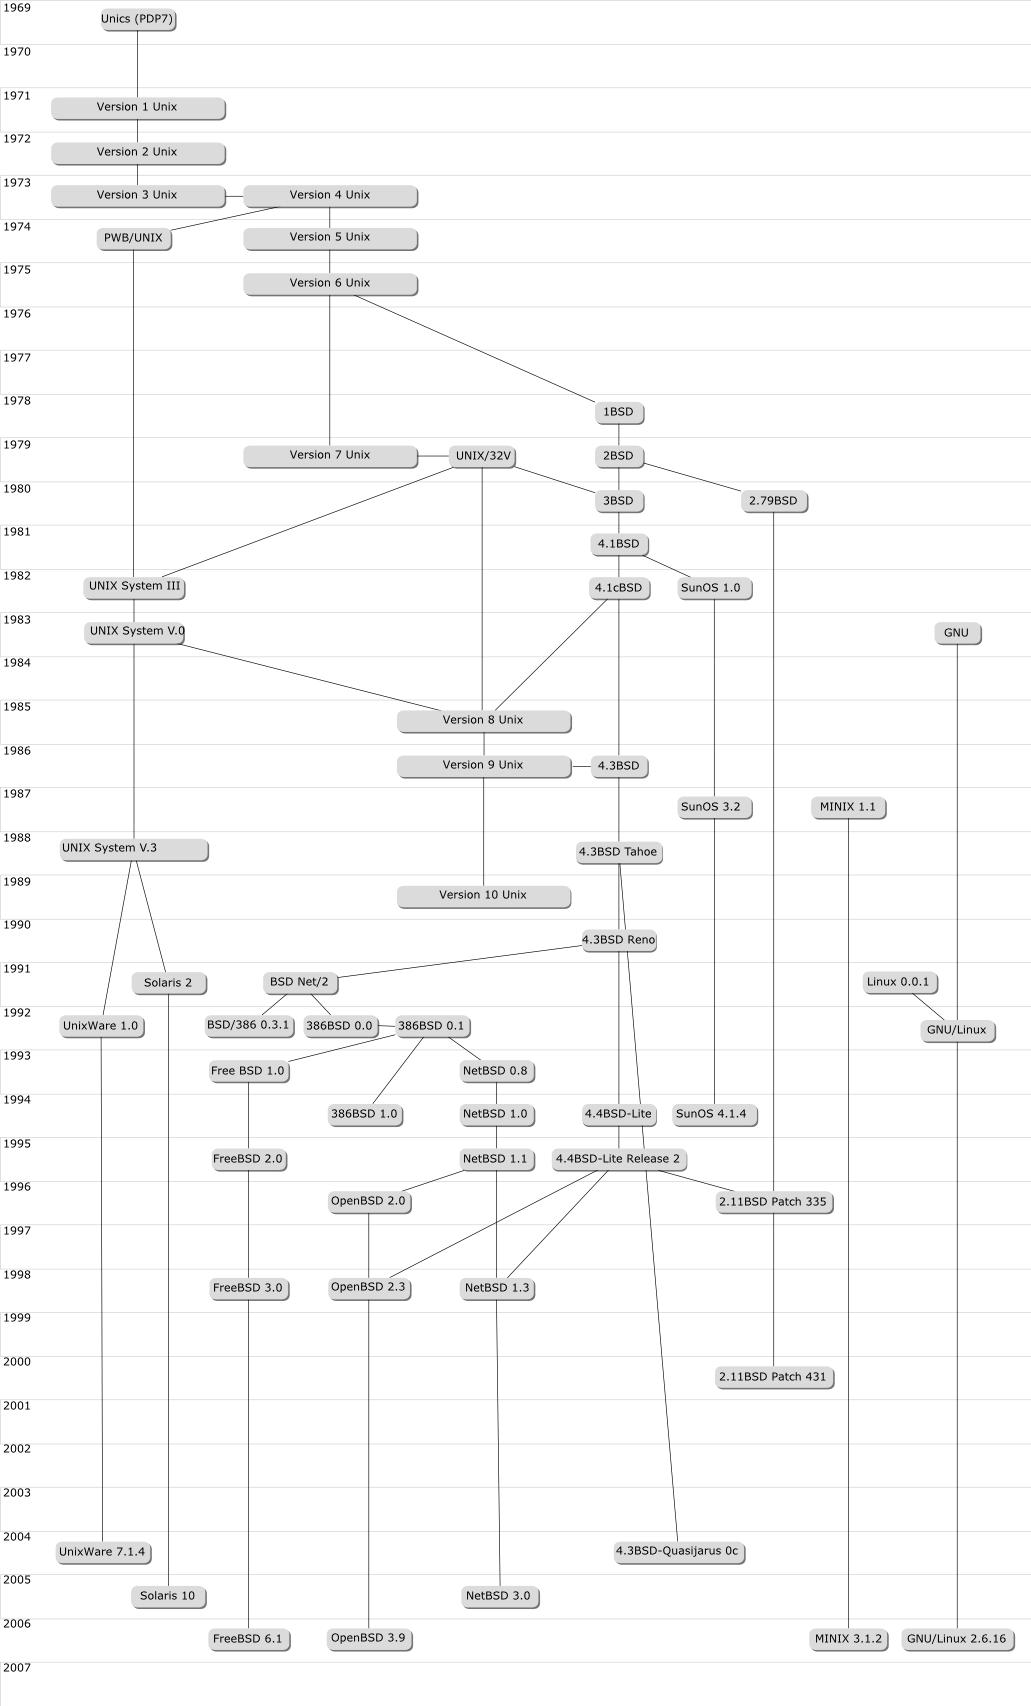
\includegraphics{pictures/unix_history}
\label{fig:unix_genealogy}
\caption{Petit historique des UNIX libres (image Wikipedia)}
\end{figure}

\section{Le langage C et la cr�ation d'UNIX}

\section{POSIX et la portabilit�}

\section{La (grande) famille BSD}


\chapter{Un petit passage par Windows}

\section{Microsoft DOS}

\paragraph{}
Anecdote sur IBM cherchant un fournisseur d'OS pour son nouveau produit : le PC

\paragraph{}
Le premier noyau de Microsoft, bas� sur DOS

\section{Les noyaux NT}

\section{Vista et 7}

\paragraph{}
Une architecture de type micro-noyau


\part{Le noyau Linux}

%%
%%
%% archi_macroscopique.tex for  in /doctorat/ece/partenariat/cours/archi_kernel
%%
%% Made by Philippe THIERRY
%% Login   <Philippe THIERRYreseau-libre.net>
%%
%% Started on  Mon Sep  6 16:18:47 2010 Philippe THIERRY
%% Last update Wed Nov 17 11:51:08 2010 Philippe THIERRY
%%

\chapter{Architecture macroscopique}

\section{La d�composition des sources}
\label{sec:decomp_sources}

\paragraph{}
\index{linux}Linux est un noyau monolithique modulaire. Il poss�de donc une grande richesse de fonctionnalit�s.\\
Le sch�ma \ref{fig:linuxmap}, tir� du site {\it makelinux}
(\url{http://www.makelinux.net/kernel\_map}), montre � quel point le noyau Linux est complexe et
difficile � apr�hender.

\paragraph{}
Les sources du noyau Linux contiennent environ dix millions de ligne de code, majoritairement �crites
en C. A la diff�rence d'un micro-noyau qui contient environ dix mille lignes de code, il est ici
n�cessaire de pr�voir une organisation des sources stricte et fine.

\paragraph{}
Dans le cadre du projet Linux, les sources sont d�compos�es par sp�cialit�s, et ce sur plusieurs
niveaux. Les sources Linux sont donc sous forme d'une arborescence de r�pertoires.

\paragraph{}
Afin de mieux comprendre les diff�rents composants pr�sent dans le noyau, le tableau \ref{tab:linux_dirs}
d�crit, pour chaque r�pertoire, les composants qui y sont h�berg�s. Ce tableau ne d�crit que le
premier niveau de r�pertoires, mais l'arbre source Linux est assez profond, pouvant descendre
jusqu'� quatre ou cinq niveaux de r�pertoires selon le type de composant. On le constate d'ailleurs
lors de l'utilisation de l'outil de configuration du noyau, qui pr�sente une arborescence assez
similaire.

\paragraph{}
\begin{center}
\tablefirsthead{\hline%
     R�pertoire & Contenu \\%
     \hline \hline}
   \tablehead{\hline \multicolumn{2}{|l|}{\small\sl suite de la page pr�c�dente}\\
   \hline  R�pertoire & Contenu\\ \hline\hline}
   \tabletail{\hline \multicolumn{2}{|r|}{\small\sl Suite page
   suivante~\ldots}\\\hline} \tablelasttail{\hline}
   \bottomcaption{R�partition des fonctionalit�s dans l'arborescence noyau Linux}
   \par
\begin{supertabular}{l|l}
\label{tab:linux_dirs}
 {\bf arch} &
 \begin{minipage}{0.7\linewidth}
 \vspace{2mm}
 Ensemble du code sp�cifique � une architecture mat�rielle donn�e. Une dizaine
 d'architecture est aujourd'hui support�e par le noyau Linux
 \vspace{2mm}
 \end{minipage}
 \\
 {\bf block} &
 \begin{minipage}{0.7\linewidth}
 \vspace{2mm}
 Impl�mentation des �l�ments g�n�riques aux p�riph�riques en mode block (disques dur, etc)
 \vspace{2mm}
 \end{minipage}
 \\

 {\bf crypto} &
 \begin{minipage}{0.7\linewidth}
 \vspace{2mm}
 Impl�mentation de l'ensemble des algorithmes cryptographiques ainsi que de la
 {\it \index{glue}glue} (On appelle {\it glue} l'ensemble des wrappers, API et macros surcouchant un c{\oe}ur
 fonctionnel) associ�e
 \vspace{2mm}
 \end{minipage}
 \\

 {\bf drivers} &
 \begin{minipage}{0.7\linewidth}
 \vspace{2mm}
 Ensemble des drivers de p�riph�rique. Ces derniers sont r�partis par famille (\index{ACPI}acpi, net,
 usb, video...)
 \vspace{2mm}
 \end{minipage}
 \\
 
 {\bf firmware} &
 \begin{minipage}{0.7\linewidth}
 \vspace{2mm}
 Ensemble des \index{firmware}firmwares et des �l�ments bas niveau n�cessaires pour s'interconnecter
 avec certains p�riph�riques.
 \vspace{2mm}
 \end{minipage}
 \\

 {\bf fs} &
 \begin{minipage}{0.7\linewidth}
 \vspace{2mm}
 Impl�mentation des diff�rents \index{filesystem}filesystems. On y retrouve \index{FS!Ext2}ext2,
 \index{FS!Ext3}ext3, \index{FS!Ext4}ext4, \index{FS!NTFS}ntfs, \index{FS!VFAT}vfat,
 \index{FS!ProcFS}procfs, \index{FS!SysFS}sysfs ou encore la sucrcouche g�n�rique � tous : \index{FS!VFS}vfs
 \vspace{2mm}
 \end{minipage}
 \\

 {\bf include} &
 \begin{minipage}{0.7\linewidth}
 \vspace{2mm}
 Ensemble des fichiers d'en-t�te du noyau export�s vers les applicatifs. Ce r�pertoire
 contient l'ensemble de l'API standard Linux.
 \vspace{2mm}
 \end{minipage}
 \\

 {\bf init} &
 \begin{minipage}{0.7\linewidth}
 \vspace{2mm}
 Dans ce r�pertoire, on retrouve l'ensemble des �l�ments n�cessaire au boot et n'�tant pas
 sp�cifique � une architecture. On retrouve ainsi la gestion de l'\index{FS!InitramFS}initramfs ou encore le montage
 du \index{RootFS}rootfs.
 \vspace{2mm}
 \end{minipage}
 \\

 {\bf ipc} &
 \begin{minipage}{0.7\linewidth}
 \vspace{2mm}
 Impl�mentation des \index{IPC}IPC \index{POSIX}POSIX (Inter-Process Communications) : les
 \index{IPC!pipe}pipes, les \index{IPC!SHM}shared-memory et les \index{IPC!Signal}signaux.
 \vspace{2mm}
 \end{minipage}
 \\

 {\bf kernel} &
 \begin{minipage}{0.7\linewidth}
 \vspace{2mm}
 Impl�mentation des �l�ments c{\oe}ur du noyau : gestion des modules, des  processus, de
 l'ordonnanceur, des \index{Access Control List}ACL \index{POSIX}POSIX ou encore des timers.
 \vspace{2mm}
 \end{minipage}
 \\

 {\bf lib} &
 \begin{minipage}{0.7\linewidth}
 \vspace{2mm}
 Ce r�pertoire contient la biblioth�que de fonctions utilis�e par l'ensemble du noyau. Il
 s'agit des fonction de base n�cessaire � l'impl�mentation de tout module Linux.
 \vspace{2mm}
 \end{minipage}
 \\

 {\bf mm} &
 \begin{minipage}{0.7\linewidth}
 \vspace{2mm}
 Impl�mentation des allocateurs m�moire de la famille mmap. Contient �galement les fonctions
 g�n�rique de gestion de la \index{MMU}MMU.
 \vspace{2mm}
 \end{minipage}
 \\

 {\bf net} &
 \begin{minipage}{0.7\linewidth}
 \vspace{2mm}
 On retrouve dans ce r�pertoire l'ensemble des piles r�seaux support�es par Linux, de la
 couche 2 � la couche 4 de la pile \index{OSI}OSI. On y retrouve la pile \index{Net!IPv4}IPv4,
 \index{Net!IPv6}IPv6, \index{Net!ATM}ATM, etc.
 \vspace{2mm}
 \end{minipage}
 \\

 {\bf security} &
 \begin{minipage}{0.7\linewidth}
 \vspace{2mm}
 Ensemble des �l�ments de durcissement standard du noyau Linux (\index{SELinux}SELinux,
 \index{Tomoyo}Tomoyo, modules \index{Trusted Plateform Module}TPM, etc).
 \vspace{2mm}
 \end{minipage}
 \\

 {\bf sound} &
 \begin{minipage}{0.7\linewidth}
 \vspace{2mm}
 Impl�mentation de l'architecture de gestion du son (hors pilotes de p�riph�riques)
 \vspace{2mm}
 \end{minipage}
 \\

 {\bf tools} &
 \begin{minipage}{0.7\linewidth}
 \vspace{2mm}
 Impl�mentation de divers outils de mesure.
 \vspace{2mm}
 \end{minipage}
 \\

{\bf scripts} &
 \begin{minipage}{0.7\linewidth}
 \vspace{2mm}
 Le r�pertoire script contient les �lements n�cessaire � la compilation du noyau. Il s'agit
 majoritairement de fichiers de scripts g�nrant certains �l�ments comme le header de version du
 noyau. Ce r�pertoire ne poss�de pas de composant source (hors headers) int�gr�s au binaire du
 noyau.
 \vspace{2mm}
 \end{minipage}
 \\

 {\bf virt} &
 \begin{minipage}{0.7\linewidth}
 \vspace{2mm}
 Support de la virtualisation. On y retrouve le sous-syst�me KVM (Kernel Virtual Machine) et
 les �lements associ�s. \index{User Mode Linux}UML (User Mode Linux), qui n'est pas de la
 \index{virtualisation}virtualisation � proprement parl�, est g�r� dans {\it arch}.
 \vspace{2mm}
 \end{minipage}
 \\
\end{supertabular}
\end{center}

\section{Linux, un noyau modulaire}
\label{sec:linux_modular}

\subsection{Principe des modules}

\paragraph{}
Linux est un noyau modulaire. Cela signifie qu'une partie de son impl�mentation peut �tre charg�e �
la vol�e, en fonction du besoin, tandis qu'une base plus petite est directement charg�e en
m�moire.\\
Le principal int�r�t et la portabilit�. En effet, les premiers blocs de code qu'on a tendance �
rendre modulable sont les pilotes. En effet, pas deux machines poss�dent exactement la m�me liste
de p�riph�rique, cependant il est n�cessaire de pouvoir installer Linux sur un maximum de machines
du parc existant. Pour cela, on int�gre dans le noyau les �l�ments de base (support du processeur,
support de la m�moire, des interruptions et des filesystems). Afin de pouvoir s'int�grer dans
diverses machine, on ajoute au noyau un nombre maximum de pilotes de p�riph�riques, sous forme de
modules. Ces pilotes tiennent de la place disque, ce qui n'est aujourd'hui pas une g�ne, mais ne
sont pas charg� en m�moire vive tant qu'ils ne sont pas n�cessaires. Cela permet ainsi de pouvoir
r�pondre � un nombre maximum de besoins sans pour autant cr�er autant de noyaux que de machines.

\paragraph{}
Cette probl�matique est moins pr�sente dans le cadre des architectures Windows. En effet, les
diff�rents pilotes de p�riph�riques sont fournis par des tiers, apr�s l'installation du noyau.
C'est aujourd'hui moins vrai, Microsoft int�grant cependant un certain nombre de pilotes g�n�riques
afin de fournir une interface utilisable avant l'installation des pilotes tiers.

\subsection{Les modules et le boot : l'\index{InitramFS}initramfs}

\paragraph{}
Sous Linux, on peut quasiment tout mettre sous forme de module. Ainsi, il est possible de
construire un noyau de base � tr�s petite empreinte m�moire, mais qui seul est insufisant pour
pouvoir initier la s�quence de boot.

\paragraph{}
C'est par exemple le cas si l'ensemble des impl�mentations de syst�mes de fichiers sont sous forme
de modules. Lorsque le noyau d�marre, il est alors incapable de charger la partition racine, le
{\it rootfs}, afin d'aller y chercher les modules n�cessaires.\\
Pour compenser ce probl�me, un syst�me de fichier virtuel a �t� cr��, le \index{FS!RamFS}ramfs, dans lequel sont
plac�s les modules n�cessaires au d�marrage de la machine. Il est cr�� sous forme d'un fichier
disjoint du fichier noyau. C'est le \index{bootloader}bootloader qui s'occupe de fournir au noyau un acc�s � ce
fichier, sans que ce dernier n'ai besoin de supporter un syst�me de fichier suppl�mentaire. Le
noyau charge alors les diff�rents modules n�cessaires au chargement de la machine, en allant lire
directement dans le fichier initramfs.\\
Initramfs est le successeur de l'\index{initrd}initrd, dont le but est le m�me, mais ayant moins de capacit�. En
effet, l'initramfs fournit plus que des modules suppl�mentaires. Il fournit �galement un rootfs
minimum, avec un shell simple, en cas de probl�me au d�but de la phase de d�marrage du syst�me.

\subsection{Le syst�me de gestion des modules et des d�pendances}

\paragraph{}
Une fois le syst�me d�marr� et le v�ritable rootfs charg�, le noyau poss�de un acc�s aux
r�pertoires de base du syst�mes que sont {\tt /bin}, {\tt /etc} et {\tt /lib}. Ces trois
r�pertoires contiennent les �l�ments n�cessaire � la poursuite du d�marrage. On y retrouve ainsi :
\begin{itemize}
\item {\bf \index{init}init}, afin de lancer le premier processus du syst�me, qui � son tour se chargera de
d�marrer les autres processus
\item {\bf \index{mount}mount}, afin de monter les possibles autres partitions du syst�me
\item les fichiers de configuration contenus dans {\bf etc}, comme la table des syst�mes de fichiers
({\tt \index{fstab}fstab}, la liste des comptes utilisateurs syst�mes fichier {\tt passwd} et d'autres �l�ments
n�cessaire � l'initiatisation du syst�me.
\item {\bf les \index{module}modules}, pr�sents dans le r�pertoire {\tt /lib}, sous forme d'une arboresence de
fichier {\tt .ko}, associ�s � des m�ta-donn�es de d�pendances.
\end{itemize}

\paragraph{}
Le noyau, en cas de besoin, est alors capable de charger � la vol�e les modules suppl�mentaire via
le syst�me de gestion des modules. Le syst�me de chargement dynamique de module se fait au travers
d'une table de correspondance. L'exemple suivant d'�crit le cas d'un p�riph�rique mat�riel:

\paragraph{}
Lorsque le noyau r�cup�re les informations sur les p�riph�riques, ces derni�res sont sous la forme
d'un couple fabriquant/identifiant. Ce syst�me est normalis�, et l'ensemble des p�riph�riques sont
capables de fournir cette indication au logiciel.\\
Lorsqu'on �crit un pilote de p�riph�rique, on pr�cise au travers de proc�dures standard du noyau
Linux la liste des p�riph�rique que le pilote sait g�rer. Cette liste contient un ensemble de
couple fabriquant/identifiant. Au moment de la compilation du noyau, lorsque le pilote est compil�
sous forme de module (et sous forme statique �galement), la liste des p�riph�riques qu'il supporte
est ajout� � la table du noyau, avec le nom du pilote. Le noyau Linux est alors capable de
connaitre quel pilote il doit charger, et par extension quel module. Il s'appuie alors sur le
syst�me de gestion des modules contenu dans le r�pertoire {\tt lib} pour trouver et charger le
module et l'ensemble de ses d�pendances si ce dernier en as. Bien entendu, c'est lors de la
compilation que les d�pendances sont ajout�es automatiquement et compil�es, afin de s'assurer de
leur pr�sence au moment de l'ex�cution.


\section{Les diff�rents �l�ments constituants le noyau Linux}
\label{sec:linux_content}

\subsection{Le support de l'architecture}

\paragraph{}
L'�l�ment principal du noyau est le support de l'architecture. Cet �l�ment est n�cessaire afin que
le noyau puisse d�marrer. Mais quels sont les �l�ments n�cessaires pour supporter l'architecture ?\\
Tout d'abord, il est n�cessaire de supporter la base : le c{\oe}ur processeur. Il est donc
n�cessaire de conna�tre ses registres et comment s'en servir. Il est �galement n�cessaire de
conna�tre les opcodes n�cessaire � la gestion des �l�ments de base comme la \index{MMU}MMU, les
\index{DMA}DMA ou encore le frequency scaling. Il est �galement n�cessaire de configurer correctement le timer, si cela n'a
pas �t� fait par le \index{bootloader}bootloader.

\paragraph{}
On retrouve ainsi dans cette partie le vecteur d'interruption et l'ensemble des handlers associ�s,
ainsi que la gestion de ces derniers (enregistrement du vecteur d'interruption, activation et
configuration du \index{PIC}PIC, etc). Sans cette configuration de base, le processeur fonctionne en vase clos
et le syst�me est inutilisable (pas de timer, pas de clavier, pas de p�riph�riques, etc).

\paragraph{}
De plus, il est n�cessaire de configurer la MMU\footnote{Memory Management Unit}, afin de passer en
mode pagin�. Cela permet de g�rer les adresses virtuel et de permettre l'emploi de la fonction {\tt
mmap}. De plus, la \index{MMU}MMU fournit un cloisonnement m�moire n�cessaire au bon fonctionnement de la
machine, via la configuration de {\it contextes} MMU par le noyau.\\
Malheureusement, il n'y a pas de norme d'interface pour la MMU, et par cons�quent il y a autant de
MMU que de processeur, d'o� sa pr�sence dans la partie support de l'architecture.

\paragraph{}
Enfin, les contr�leurs \index{DMA}DMA ma�tre, souvent pr�sents directement dans le processeur, doivent �tre
configur�s. Pour finir, le support du bus \index{PCI}PCI et au travers de lui la d�couverte des p�riph�riques
est g�r� �galement dans cette partie.

\subsection{La gestion m�moire}
\paragraph{}
La MMU est g�r�e dans le support de l'architecture. Cependant, d'un point de vue plus
macroscopique, il est n�cessaire de g�rer les pages et la m�moire vive. Il faut donc impl�menter
une ou des politiques d'allocation m�moire (nomm�es dans Linux {\it slub}et {\it slab allocators}.
De plus, lors de la construction d'un processus et de la configuration de son contexte MMU, le
positionnement des sections et la configuration de l'espace d'adressage doit �tre fait. C'est dans
cette partie que sont g�r�s ces diff�rents �l�ments.

\subsection{Le gestionnaire d'interruptions}
\paragraph{}
Il est d�crit dans la partie support de l'architecture que la pr�sence d'un vecteur d'interruption
est n�cessaire, et que le noyau doit enregistrer se dernier aupr�s du processeur. Le vecteur
d'interruption est en g�n�ral une liste d'adresses. Dans le cas des processeurs de la famille
\index{IA32}IA32,
ce vecteur poss�de une longueur de 256 adresses. On retrouve 16 cases pour les interruptions
mat�rielles, 128 cases pour les interruptions logicielles, et le reste en r�serve. Cependant,
chaque adresse correspond � la position d'une fonction en m�moire, cette fonction �tant sp�cialis�e
pour l'interruption associ�e. Ces fonctions sont toutes impl�ment�es dans le noyau Linux et
n�cessite parfois l'appel � un pilote externe, comme par exemple le gestionnaire d'interruption
clavier, qui n�cessite... un pilote clavier.\\
On retrouve �galement les handlers d'exception mat�rielles et logicielles, dont toute une partie de
l'impl�mentation n'est pas sp�cifique au mat�riel, mais relatif � la politique de Linux. Ainsi, l�
o� une exception de type page-miss implique une mise � jour de l'arborescence de page du processus
associ� via requ�te � la MMU, une exception de type division par z�ro implique la terminaison du
processus en cause.

\subsection{Les \index{syscall}syscalls}
\paragraph{}
Dans les deni�res versions du noyau 2.6 (version 2.6.35), Linux poss�de une cinquantaine de
syscalls. Ces derniers sont directement appellable par les processus userspace. Leur appel est
directement remplac� par la cha�ne de compilation par une requ�te d'interruption 80. Cette
interruption, g�r�e dans le vecteur d'interruption, redirige vers l'appel syst�me associ� en
fonction de la valeur de certains registres, mise � jour plus haut dans le code assembleur de la
t�che.

\paragraph{}
La plupart du temps, les syscall fournissent une inerface d'�change de donn�es entre le processus
et le noyau, via un buffer. C'est le cas de l'appel syst�me {\tt read}, dont le prototype est le
suivant :
\begin{lstlisting}
ssize_t	read(int fd, char *buf, size_t count);
\end{lstlisting}

\paragraph{}
En g�n�ral, les appels syst�mes sont d�compos�s en plusieurs blocs. Le premier bloc est propre au
coeur du noyau Linux, et prend en charge les �l�ments g�n�riques. Ainsi, dans le cadre du read, ce
dernier v�rifie que fd existe bien dans la table des descripteurs de fichiers.

\paragraph{}
Un descripteur de fichier est un entier auquel est associ� un fichier dans le syst�me de fichiers.
Il est alors n�cessaire de passer la main on second bloc, impl�ment� dans le pilote du syst�me de
fichier virtuel {\tt vfs}. Ce dernier est une interface homog�ne pour l'ensemble des syst�mes de
fichiers sous jacents, et il y en a beaucoup. Ainsi, si le fichier se trouve dans une partition
ext3, ce bloc passe la main � l'impl�mentation du read du pilote de l'ext3, si c'est dans le
procfs, il passe alors la main au pilote du procfs, si c'est dans le devfs ({\tt /dev}), alors le
troisi�me bloc appell� est le pilote du {\it devfs}.\\
Dans certain cas, ce troisi�me bloc est le dernier. C'est le cas par exemple des pilotes de
syst�mes de fichiers physiques (syst�mes de fichiers des partitions disques). Cependant, dans le
cas des syst�mes de fichiers virtuel, un autre driver se cache encore en dessous.\\
C'est le cas par exemple pour {\it devfs}. Ce dernier passe alors la main � l'impl�mentation du
pilote de p�riph�rique associ� au fichier device.

\paragraph{}
On constate que l'impl�mentation des appels syst�mes est stratifi�. Cela permet de mieux ma�triser
les diff�rentes �tapes du traitement, mais implique une consommation en terme de cycles processeur.
Fort heureusement, l'ex�cution de l'appel syst�me se fait dans l'espace d'adressage du processus
appelant. Cela �vite ainsi un changement de contexte. Cependant, un changement de niveau de
privil�ge doit �tre effectu�, l'appel syst�me se faisant avec les droits du noyau.\\
Afin de rendre ces deux propri�t�s compatibles, une partie de la section de code du noyau est
pr�mapp�e dans l'espace d'adressage du noyau, ce qui permet d'appeller les diff�rentes fonctions du
noyau via un simple branchement, apr�s changement de niveaux de privil�ge.

\subsection{Les IPC}
\paragraph{}
Linux impl�mente les IPC POSIX. Il s'agit des trois suivantes :
\begin{itemize}
\item Les signaux, permettant de communiquer de mani�re simple au travers de l'impl�mentation de
handlers de signaux au niveau logiciel. Parmis ces signaux, trois (\FIXME � v�rifier) ne sont pas
red�finissable par une tache : \index{IPC!Signaux!SIGKILL}SIGKILL et \index{IPC!Signaux!SIGTERM}SIGTERM et
\index{IPC!Signaux!SIGILL}SIGILL. Ces signaux provoque la terminaison
de la tache cible. Un signal n'est qu'une valeur num�rique. Elle ne contient aucune autre
information que sa valeur.
\item Les pipes, fournissant un canal de communication unidirectionnel. Les pipes �tant vus sous
formes de descripteurs de fichiers partag�s entre deux taches, ces derni�res doivent �tre cr��es
par une m�me tache parente, responsable de la cr�ation du pipe en avance de phase.
\item Les m�moire partag�es. Il s'agit de la famille {\it shm}. Il s'agit de page m�moires (dont la
granularit� est g�n�ralement de 4096 octets) que deux processus partagent. L'�criture ou la lecture
dans cette page m�moire se fait au travers des fonctions de la famille {\it shm} comme {\tt shmget}.
\end{itemize}

Il existe d'autre moyens de communiquer entre processus, comme par exemple au travers d'une
\index{socket}socket
UNIX, mais il ne s'agit pas, dans ce cas, d'une \index{IPC}IPC.

\subsection{L'ordonnanceur et la gestion des taches}

\paragraph{}
Un noyau doit imp�rativement g�rer des taches, faute de quoi sont int�r�t serait fortement r�duit.
POSIX fournit un certain nombre de propri�t�s qu'une tache doit poss�der :
\begin{itemize}
\item un identifiant, nomm� {\it \index{Pid}pid} (Process IDentifier)
\item une tache parente, connue via son identifiant, le {\it ppid} (Parent Process IDentifier)
\item un utilisateur propri�taire de la tache, d�finissant un userid associ�, et en cons�quence
      ses droit d'acc�s utilisateur.
\item un groupe propri�taire de la tache, d�finissant un groupid associ�, et ses droit d'acc�s
      groupe.
\item une politique d'ordonnancement, pouvant �tre de type RR (Round Robin), FIFO, ou encore OTHER)
\item une priorit�, afin de l'int�grer dans sa politique d'ordonnancement
\item un age, pouvant avoir un impact sur sa priorit�, au travers de la gestion du vieillissement
      des taches.
\item sa priorit� modifi�e, nomm�e priorit� {\it nice}, cons�quence du vieillissement mais
      �galement d'une possible red�finition de sa priorit� via la commande {\tt nice}.
\item un contexte MMU, correspondant � un identifiant d'espace d'adressage, afin de savoir quel
      espace charger au moment de son ordonnancement.
\item un tableau de descripteur de fichier, listant l'ensemble des file descriptors et des fichiers
      associ�s ouvert, ainsi que les droits demand�s � l'ouverture
\item Quelques propri�t�s en terme de charge maximum, comme le nombre de file descriptors maximum
      ouvrable.
\end{itemize}

\paragraph{}
Une tache poss�de d'autres propri�t�s, mais celles nomm�es ici sont les principales. On constate
donc qu'une tache est un �l�ment complexe, n�cessitant une grosse structure de donn�e, ainsi qu'une
interface riche de gestion de tache.

\paragraph{}
Qui dit tache dit bien sur ordonnanceur. Linux poss�de de base plusieurs types d'ordonnanceurs. Il
poss�de tout d'abord des ordonnanceurs temps r�el (FIFO et RR), mais �galement non-temps r�el. A
ses ordonnanceur sont associ�es des priorit�s:
\begin{enumerate}
\item 100 priorit�s diff�rentes pour les ordonnanceurs temps r�el, de 0 (la plus basse) � 99
\item 40 priorit�s pour les ordonnanceurs non temps r�el, de 20 (la plus basse), � -19.
\end{enumerate}
Cela fait au total 140 priorit�s � g�rer. Le fait qu'il y aie plusieurs ordonnanceurs s'ex�cutant en
m�me temps, le syst�me d'ordonnancement de Linux est assez complexe. Cependant, depuis le noyau
2.6.11, l'ordonnanceur standard pour le non temps r�el ({\it SCED\_OTHER}) poss�de une complexit�
en $O(1)$. Avec l'accroissement du nombre de taches s'ex�cutant en parall�le sur une machine,
s'�tait une n�cessit�.

\paragraph{}
De plus, afin d'�viter les locks li�s aux architectures multi-c{\oe}urs, Linux est pass� d'une file
unique de gestion des taches � une file par c{\oe}ur. Cela �vite que deux instance de
l'ordonnanceur s'ex�cutant en parall�le g�n�re un retard sur l'une d'entre elle.

\subsection{Les syst�mes de fichiers}
\paragraph{}
La gestion des syst�mes de fichiers sous Linux fonctionne en couche. Le but est que du point de vue
utilisateur, un seul syst�me de fichier ne soit vu. Cela permet de fournir aux applications une
interface d'acc�s unique et homog�ne.\\
Le sch�ma \ref{fig:fs_archi} fournit un exemple d'architecture en couche telle que pr�sente dans
Linux. Ce sch�ma n'est pas exhaustif : il existe d'autres syst�mes de fichiers non pr�sent�s ici
comme le {\it NTFS} ou encore, parmi les syst�mes de fichiers virtuels, les {\it sysfs}, {\it ramfs}
et {\it tmpfs}, mais le principe de fonctionnement reste le m�me pour tous, avec un acc�s au travers
du vfs.

\begin{center}
\begin{figure}[H]
%%
%%
%% fs_archi.tex for  in /doctorat/ece/partenariat/cours/archi_kernel
%%
%% Made by Philippe THIERRY
%% Login   <Philippe THIERRYreseau-libre.net>
%%
%% Started on  Fri Oct  1 11:09:45 2010 Philippe THIERRY
%% Last update Fri Oct  1 11:40:38 2010 Philippe THIERRY
%%

\begin{pdfpic}
\scalebox{1}{
\begin{pspicture}(0,0)(12,7)
\psline{-}(0,0)(0,0)
\definecolor{RootFS}{rgb}{0,0,0.4}
%--- rootfs
\psframe[linewidth=0.04cm,fillstyle=solid,fillcolor=RootFS,framearc=.3](1,5)(15,6) % shadow
\rput(3,5.6){\text \color{white}{/, /etc, /boot, /bin}}
\rput(3,5.2){\text \color{white}{/usr, /var, /tmp, /home}}
%--- VFS
\definecolor{VFS}{rgb}{0,0,0.7}
\psframe[linewidth=0.04cm,fillstyle=solid,fillcolor=VFS,framearc=.3](1,4)(15,5) % shadow
\rput(8,4.5){\text \color{white}{Virtual File System}}
%--- EXT3
\definecolor{EXTFS}{rgb}{0,0.7,0}
\psframe[linewidth=0.04cm,fillstyle=solid,fillcolor=EXTFS,framearc=.3](1,3)(5,4) % shadow
\rput(3,3.5){\text \color{white}{EXT3fs, EXT4fs, VFS...}}
% bellow ext3fs
\definecolor{Drivers}{rgb}{0.4,0,0.4}
\psframe[linewidth=0.04cm,fillstyle=solid,fillcolor=Drivers,framearc=.3](1,2)(5,3) % shadow
\rput(3,2.5){\text \color{white}{mass storage driver}}
%--- PROCFS
\rput(6,5.4){\text \color{white}{/proc}}
\definecolor{EXTFS}{rgb}{0.7,0,0}
\psframe[linewidth=0.04cm,fillstyle=solid,fillcolor=EXTFS,framearc=.3](5,3)(7,4) % shadow
\rput(6,3.5){\text \color{white}{ProcFS}}
% bellow procfs
\psframe[linewidth=0.04cm,fillstyle=solid,fillcolor=Drivers,framearc=.3](5,2)(7,3) % shadow
\rput(6,2.5){\text \color{white}{drivers}}
%--- DEVFS
\rput(8,5.4){\text \color{white}{/dev}}
\psframe[linewidth=0.04cm,fillstyle=solid,fillcolor=Drivers,framearc=.3](7,3)(9,4) % shadow
\rput(8,3.5){\text \color{white}{drivers}}
%--- iso9660
\rput(10.5,5.4){\text \color{white}{/media/cdrom}}
\definecolor{ISO9660}{rgb}{0,0.4,0.4}
\psframe[linewidth=0.04cm,fillstyle=solid,fillcolor=EXTFS,framearc=.3](9,3)(12,4) % shadow
\rput(10.5,3.5){\text \color{white}{ISO9660}}
% bellow iso9660
\psframe[linewidth=0.04cm,fillstyle=solid,fillcolor=Drivers,framearc=.3](9,2)(12,3) % shadow
\rput(10.5,2.5){\text \color{white}{Cdrom driver}}
%--- USB storage (vfat)
\rput(13.5,5.4){\text \color{white}{/media/usb}}
\definecolor{VFat}{rgb}{0.4,0.4,0}
\psframe[linewidth=0.04cm,fillstyle=solid,fillcolor=VFat,framearc=.3](12,3)(15,4) % shadow
\rput(13.5,3.5){\text \color{white}{VFat}}
% bellow iso9660
\definecolor{USBStack}{rgb}{0,0.2,0.2}
\psframe[linewidth=0.04cm,fillstyle=solid,fillcolor=Drivers,framearc=.3](12,2)(15,3) % shadow
\rput(13.5,2.5){\text \color{white}{USB Mass storage}}
\psframe[linewidth=0.04cm,fillstyle=solid,fillcolor=USBStack,framearc=.3](12,1)(15,2) % shadow
\rput(13.5,1.5){\text \color{white}{USB Stack}}



\end{pspicture}
}
\end{pdfpic}

\caption{Architecture en couche de la gestion des syst�mes de fichiers}
\label{fig:fs_archi}
\end{figure}
\end{center}

\subsection{La pile r�seau}

\paragraph{}
La pile r�seau Linux est tr�s riche et ne se limite pas au seul couple Ethernet/IP. On y retrouve
�galement un certain nombre de protocoles legacy comme ATM, TDMA ou encore TokenRing, ainsi que le
support des normes IEEE 802.11, 802.15.4, etc. Du fait de sa richesse, la pile r�seau Linux est
tr�s complexe. Sont d�crit ici les structures principales, dans le cadre de la pile IP.

\paragraph{}
Afin d'exploiter au mieux les capacit�s r�seau de Linux, il existe un composant, assez volumineux
(environ cent mille lignes de code) nomm� {\it Netfilter}. Ce composant est ce qu'on appelle un
treillis: il accompagne le traitement du flux r�seau dans le noyau, et propose des accroche
permettant d'effectuer des traitements sp�cifique � divers moment du cheminement des paquets dans
la pile r�seau.

\paragraph{}
Pour comprendre l'architecture de Netfilter il est avant tout n�cessaire de bien avoir en t�te la pile
IP, et sa d�composition entre le noyau et le mode utilisateur. Pour rappel, le traitement des
en-t�tes s'effectue dans le noyau jusqu'� la couche 4 du mod�le OSI. C'est ensuite � l'applicatif
de traiter le reste du paquet.
La liaison entre noyau et userspace se fait, dans le cadre d'un environnement POSIX comme Linux,
via des sockets. Netfilter n'intervient que dans la partie noyau, mais peut parfois remonter plus
haut que la couche 4, c'est ce qu'on appelle le conntracking. Son usage est d�crit plus loin.

\paragraph{}
Avant que le paquet n'arrive au niveau de la couche liaison de la pile IP, il a d�j� parcouru du
chemin dans le noyau Linux. En effet, ce dernier a �t� charg� � partir de la m�moire de la carte r�seau,
et structur� de mani�re standardis�e dans une structure propre au noyau Linux appel�e {\it
sk\_buff}.\\
Cette structure contient un certain nombre d'informations sur le paquet, comme par exemple :
\begin{itemize}
\item Sa taille
\item Son interface d'entr�e (pointeur vers la stucture {\it net\_device} correspondante du noyau)
\item Son interface de sortie (champ remplit au moment du routage du paquet si sa destination n'est
      pas locale)
\item Sa date d'arriv�e
\item Des pointeurs divers vers les en-t�tes liaison et IP, ainsi que vers la fin du paquet
\item la somme de contr�le du paquet
\item Sa priorit�
\end{itemize}

\paragraph{}
Linux est capable de forwarder du flux, au niveau liaison (bridging) et au niveau r�seau (routing).
Le flux est alors d�capsul� respectivement jusqu'� la couche liaison et jusqu'� la couche r�seau.
Cela permet de diriger se dernier vers la bonne interface, et si besoin de construire une en-t�te
diff�rente de la pr�c�dente (cas du bridging, avec changement de MAC source, du DNAT, du SNAT, et
du MASQUERADING), voire de changer de protocole de niveau liaison ou transport. Linux agit alors comme une
gateway.

\paragraph{}
Il est �galement possible de modifier le chemin pr�vu dans le datagramme (proxying, etc). On parle
alors dans ces cas l� de "paquet mangling", puisque l'on va modifier des champs dans les en-t�tes.
Sont �galement modifi�s des champs comme le TTL, et un possible re-d�coupage des datagrammes peut
�tre fait, selon les sp�cification du r�seau de sortie.

\paragraph{}
Ce traitement doit se faire de mani�re rapide afin de limiter la latence de transit, et doit pouvoir
�tre ordonnanc� en fonction des besoins du r�seau. Il s'agit d'une probl�matique complexe sur la
qualit� de service induite par la latence. Une solution a �t� mise en place sous Linux, d�crite
plus loin.

\paragraph{}
Netfilter est la pierre angulaire de tous ces traitements. Ce n'est pas lui qui impl�mente les
fonctions de la pile IP, mais il ordonnance leurs appels, en fonction des valeurs qu'elles retournent,
et selon les informations fournies par les {\it sk\_buffs}.

\paragraph{}
Netfilter s'appuie sur un sch�ma g�n�rique de traitement des paquets. Il d�finit 5 traitements
successifs au niveau IP :
\begin{itemize}
\item NF\_IP\_PREROUTING, qui va faire un traitement pr�alable au routage du paquet.
      C'est ici qu'iptables g�re le DNAT par exemple. Ce traitement ce fait � l'arriv�e des paquet en entr�e
\item NF\_IP\_IN, pour le traitement avant la remont�e vers la socket locale du paquet.
      Ce hook est utilis� pour la finalisation du traitement des paquets entrant.
\item NF\_IP\_FORWARD, pour le forwarding de paquet uniquement. C'est cette accroche qui va appeler
      le module de routage du noyau (traitement de la table de routage)
\item NF\_IP\_OUT, pour le pr�-traitement des paquets en �mission � partir d'une source locale
      uniquement.
\item NF\_IP\_POSTROUTING, pour le post-traitement du paquet en �mission. Ex�cut� � la fois lors du routage
      et lors de l'�mission de paquets depuis un service local. On y trouve par exemple les r�gles
      d'encapsulation IPSEC pour le mode tunnel. C'est le dernier � �tre appel� avant �mission du paquet.
\end{itemize}
Ces cinq traitements sont �galement pr�sents au niveau liaison, afin de r�pondre au besoin de
bridging. Cependant, NF\_BR\_PREROUTING et NF\_BR\_POSTROUTING sont constamment appel�s. Le sch�ma
\ref{fig:nf_hooks} d�crit le positionnement des diff�rentes accroches Netfilter.

\begin{figure}
%%
%%
%% nf_hooks.tex for  in /doctorat/ece/partenariat/cours/archi_kernel
%%
%% Made by Philippe THIERRY
%% Login   <Philippe THIERRYreseau-libre.net>
%%
%% Started on  Fri Oct  1 13:35:49 2010 Philippe THIERRY
%% Last update ven. 15 avril 2011 15:33:52 CEST Philippe THIERRY
%%

\begin{pdfpic}
\scalebox{0.75}{
\begin{pspicture}(-1,-1)(20,8)
\definecolor{NF}{rgb}{0.7,1,1}
% incoming NIC
\psframe[linewidth=0.04cm](0,0)(1,0.7)
\psframe[linewidth=0.03cm](0.2,0.2)(0.6,0.5)
\psline[linewidth=0.06cm](1,0)(1,1)(1.1,1)
\rput[rt](0.5,-0.2){\text NIC}
% ISR and poller
\psframe[linewidth=0.04cm](2,2)(3,2.5)
\rput(2.5,2.25){\text ISR}
\psframe[linewidth=0.04cm](2,3.5)(3,4)
\rput(2.5,3.75){\text Poller}
% link from NIC to ISR & poller
\psline[linewidth=0.04cm]{->}(0.5,0.7)(2,2.25)
\psline[linewidth=0.04cm]{->}(0.5,0.7)(2,3.75)
% first temporal break
\psline[linewidth=0.04cm]{->}(3,2.25)(4,2.25)
\psline[linewidth=0.04cm]{->}(3,3.75)(4,3.75)
\psline[linewidth=0.04cm](4,1.5)(4,4.5)
\rput(4.25,3){\rotatebox{90}{\text first temporal break}}
\psline[linewidth=0.04cm](4.5,1.5)(4.5,4.5)
% L2 first pass
\psframe[linewidth=0.04cm](4.5,2)(6.5,3)
\rput(5.5,2.6){\text L2}
\rput(5.5,2.3){\text prerouting}
% In
\psline[linewidth=0.04cm](9,6)(8,6)(8,7)(9,7)
% ip prerouting
\psframe[linewidth=0.04cm](7.5,4)(9.5,5)
\rput(8.5,4.6){\text IP}
\rput(8.5,4.3){\text Prerouting}
% ip forwarder
\psframe[linewidth=0.04cm](10,4)(12,5)
\rput(11,4.6){\text IP}
\rput(11,4.3){\text Forwarder}
% briding
\psframe[linewidth=0.04cm](7.5,2)(14.5,3)
\rput(11,2.5){\text Bridging}
% links from L2 first pass
\psline[linewidth=0.04cm]{->}(6.5,2.5)(7.5,2.5)
\psline[linewidth=0.04cm]{->}(6.5,3)(7.5,4.5)
\psline[linewidth=0.04cm]{->}(9.5,4.5)(10,4.5)
\psline[linewidth=0.04cm]{->}(8.5,5)(8.5,6)
% out
\psline[linewidth=0.04cm](13,6)(14,6)(14,7)(13,7)
\psline[linewidth=0.04cm]{->}(13.5,6)(13.5,5)
% ip postrouting
\psframe[linewidth=0.04cm](12.5,4)(14.5,5)
\rput(13.5,4.6){\text IP}
\rput(13.5,4.3){\text postrouting}
\psline[linewidth=0.04cm]{->}(12,4.5)(12.5,4.5)
% br postrouting
\psframe[linewidth=0.04cm](15.5,2)(17.5,3)
\rput(16.5,2.6){\text L2}
\rput(16.5,2.3){\text postrouting}
\psline[linewidth=0.04cm]{->}(14.5,4)(16.5,3)
% second temporal break
\psline[linewidth=0.04cm](17.5,1.5)(17.5,4.5)
\rput(17.75,3){\rotatebox{90}{\text second temporal break}}
\psline[linewidth=0.04cm](18,1.5)(18,4.5)
% output queue 1
\psframe[linewidth=0.04cm](18.3,2)(18.7,3)
\psline[linewidth=0.04cm](18.3,2.2)(18.7,2.2)
\psline[linewidth=0.04cm](18.3,2.4)(18.7,2.4)
\psline[linewidth=0.04cm](18.3,2.6)(18.7,2.6)
\psline[linewidth=0.04cm](18.3,2.8)(18.7,2.8)
% output queue 2
\psframe[linewidth=0.04cm](18.9,2)(19.3,2.8)
\psline[linewidth=0.04cm](18.9,2.2)(19.3,2.2)
\psline[linewidth=0.04cm](18.9,2.4)(19.3,2.4)
\psline[linewidth=0.04cm](18.9,2.6)(19.3,2.6)
% output NIC
\psframe[linewidth=0.04cm](18.3,0)(19.3,0.7)
\psframe[linewidth=0.03cm](18.5,0.2)(18.9,0.5)
\psline[linewidth=0.06cm](19.3,0)(19.3,1)(19.4,1)
\rput(18.8,-0.2){\text NIC}
% Let's mark the NF hooks now
\psline[linewidth=0.06cm,linecolor=red]{<-}(5.5,2)(5.5,0)
\rput(5.5,-0.3){\text {\color{red}{NF\_BR\_PREROUTING}}}
\end{pspicture}
}
\end{pdfpic}

\label{fig:nf_hooks}
\caption{Positionnement des diff�rentes accroches Netfilter sur la pile IP}
\end{figure}

\paragraph{}
Des exemples de services se basant sur les hooks de Netfilter sont les services de conntracking.
Un certain nombre de protocoles de niveau sup�rieur � la couche transport utilise plusieurs ports
pour fonctionner, en choisissant un port � la vol�e, durant une p�riode d'initialisation. C'est
le cas du protocole FTP, sur le port 21, qui choisit dynamiquement un port pour �mettre des donn�es
binaires tout en maintenant le port 21 ouvert pour la signalisation.\\
Cependant, lorsqu'un firewall est actif sur la machine, on croit souvent �tre oblig� de configurer
une plage de ports ouverts de mani�re statique afin de permettre ce cas d'emploi.
En r�alit�, il existe un module dans le noyau linux, qui s'accroche � Netfilter et qui va traiter
le protocole FTP dans le noyau, � la vol�e. Il d�capsule le flux jusqu'� arriver au niveau du flux
FTP, afin de d�tecter la n�gociation de port. Une fois le port n�goci�, le module ouvre le port �
la vol�e entre le client et le serveur, ce qui permet au flux de donn�es de traverse.

\paragraph{}
Il existe aujourd'hui un grand nombre de module de conntracking, allant du support du protocole FTP au
support des protocole SIP et H323.

\subsection{La pile USB}

\paragraph{}
L'architecture USB est un bloc volumineux de Linux. En effet, entre les diff�rentes normes (OHCI et
UHCI pour l'USB 1.1, EHCI pour l'USB 2 et l'XHCI pour l'USB 3.0), les diff�rents modes associ�s
(mode Interrupt, Bulk, etc) et les diff�rents types de p�riph�riques pouvant s'y connecter (disques
durs, cam�ra, contr�leurs r�seau (ethernet ou Wifi), claviers, souris, etc.), le sous-syst�me USB
est tr�s consommateur � la fois de d�veloppeurs et de modules.

\paragraph{}
La pile USB Linux reprend, pour la d�nomination de ses structures et ses champs, les noms d�finis
dans les normes associ�es, ce qui simplifie l'usage des API.\\
L'�l�ment de base le plus fr�quement utilis� dans le cadre des communications avec les
p�riph�riques USB est l'{\it URB}. Il s'agit d'une structure de donn�es faisant office de support
dans la communication entre pilote et p�riph�rique. On peut le voir comme l'�quivalent du {\it
sk\_buff} pour les interfaces r�seaux.

\paragraph{}
Sous Linux, le syst�me USB est vu comme un arbre. Les noeuds sont les hubs USB, g�r�s nativement
par le noyau via un thread sp�cifique nomm� {\it khubd}. Ce d�mon est la porte de sortie des
diff�rents �v�nements p�riph�riques transitant par les hubs. C'est lui qui informe alors le noyau
qu'un �v�nement a eu lieu, et appelle le driver associ�. {\it Khubd} est en attente d'�v�nement au
travers d'un m�canisme de polling, dont la p�riode est une propri�t� fournie par le controlleur USB
mat�riel.

\paragraph{}
L'impl�mentation de la pile USB commence � se stabiliser ces deux derni�res ann�es. Elle reste
cependant tr�s dynamique, du fait de l'arriv�e de la norme USB 3 et de la constante int�gration de
nouveaux p�riph�riques USB.

\subsection{La s�curit� et la cryptographie}
\paragraph{}
Le noyau Linux fournit un certain nombre de service de base, comme le support des droits POSIX
(support des utilisateurs et des groupes, sur une valeur octale allant de 000 � 777),
avec une politique de s�curit� de type DAC\footnote{Discretionary Access Control} et le support des
{\it capabilities} POSIX.\\
Les capabilities d�finissent des classes de privil�ges avec le support de l'h�ritage des privil�ges
lors de la cr�ation d'un processus fils).\\
\`{A} cela est ajout� le support des droits �tendus (flags setuid, setgid, etc).

\paragraph{}
La gestion des droits telle que d�finie ci-dessus est toujours pr�sente dans un noyau Linux, quel
que soit sa configuration (hors capabilities, qui peut �tre d�sactiv�). Cependant, il existe
plusieurs modules compl�mentaires permettant d'int�grer des fonctions de s�curit� suppl�mentaires.
Il s'agit des �l�ments suivants :\\
\begin{itemize}
\item {\bf SELinux}: introduit par la NSA, ce module fournit un support du mode
RBAC\footnote{Role-Based Access Control} permettant de d�finir des r�les et des droits pour chacun
deux. Contrairement au DAC, ce n'est plus l'utilisateur qui d�finit ses droits (et ceux de ses
fichiers) mais la politique de s�curit� associ� au mod�le RBAC.
\item {\bf SMAC}: Il s'agit d'un module int�gr� r�cement, dont le but et de supporter un mod�le de
s�curit� de type MAC\footnote{Mandatory Access Control} simplifi�. Il s'agit de d�finir de mani�re
statique des droit pour les diff�rents utilisateurs en terme de visibilit� sur le syst�me et sur
les acc�s qu'il a le droit de faire. Il s'agit d'un mod�le plus simple � g�rer que le RBAC, mais
moins pr�cis.
\item {\bf AppArmor}: Module int�gr� dans le noyau Linux par Canonical (distribution Ubuntu) qui
s'en sert dans sa distibution. Il fournit le support d'un mod�le RBAC avec support de
l'apprentissage, proche de SELinux.
\item {\bf les TPM}: Support des Trusted Plateform Modules. Pemet de prendre en compte certains
�l�ments mat�riel de s�curisation.
\end{itemize}

\paragraph{}
Linux impl�mente un certain nombre d'algorithme de chiffrement et de hachage, comme le SHA1, l'AES
ou encore le DES. Ces diff�rents algorithmes sont employ�s au niveau du noyau pour la
gestion de l'IPSEC ou des syst�mes de fichiers chiffr�s par exemple. Ils sont �galement accessible
aux applicatifs au travers de l'API du noyau.

\subsection{Les pilotes de p�riph�riques}
\paragraph{}
Comme vu dans le cas de l'USB, Linux impl�mente un grand nombre de pilote de p�riph�rique. Ces
derniers sont classifi�s en fonction de leur famille (net devices, usb, char devices, block
devices...). \`{A} chaque famille est associ�e une liste de pilotes dans laquelle Linux va piocher
lors de la d�couverte des p�riph�riques.\\
Un pilote de p�riph�rique fournit l'interface entre le noyau et le mat�riel qu'il g�re. Il doit
donc s'enregistrer aupr�s du noyau pour lui preciser quel mat�riel il supporte, et comment le noyau
doit se servir de lui. Chaque famille poss�de une interface standardis�e qui permet au pilote
d'enregistrer les diff�rentes fonctions de son API aupr�s du noyau.\\
Pour d�finir les p�riph�riques qu'un pilote supporte, le noyau s'appuie sur un syst�me normalis� de
couple constructeur/mod�le. Il s'agit de deux valeur num�rique que chaque p�riph�rique est capable
de donner de mani�re g�n�rique. Lorsqu'un pilote donne au noyau la liste des p�riph�rique qu'il
supporte, il fournit la liste des couples constructeur/mod�le qu'il sait g�rer. Ce couple est bien
sur unique pour un mod�le donn�. Pour pouvoir poss�der un num�ro de constructeur, la soci�t� doit
s'enregistrer aupr�s d'instances internationales.

%%
%%
%% archi_production.tex for  in /doctorat/ece/partenariat/cours/archi_kernel
%%
%% Made by Philippe THIERRY
%% Login   <Philippe THIERRYreseau-libre.net>
%%
%% Started on  Mon Sep  6 16:28:58 2010 Philippe THIERRY
%% Last update Mon Sep  6 16:30:26 2010 Philippe THIERRY
%%

\chapter{Le syst�me de production du noyau}

\section{La structure de Makefiles}

\section{Les fichiers KConfig et l'interface de configuration}

\subsection{La syntaxe des KConfig}

\subsection{Les d�pendances inter-modules}


%%
%%
%% archi_microscropique.tex for  in /doctorat/ece/partenariat/cours/archi_kernel
%%
%% Made by Philippe THIERRY
%% Login   <Philippe THIERRYreseau-libre.net>
%%
%% Started on  Mon Sep  6 16:26:28 2010 Philippe THIERRY
%% Last update Mon Sep  6 16:28:07 2010 Philippe THIERRY
%%

\chapter{Architecture avanc�e}

\section{Les interfaces noyau pour les modules}

\subsection{Les fonctions et macros g�n�ralistes}
\paragraph{}

\subsection{Les structures de donn�es et leurs accesseurs}
\paragraph{}

\subsection{Cr�er et syncrhoniser des threads noyau}

\subsubsection{Les tasklets}
\paragraph{}

\subsubsection{Les timers}
\paragraph{}



\part{Annexes}

\begin{appendices}
%%
%%
%% annexe_linuxmap.tex for  in /doctorat/ece/partenariat/cours/archi_kernel
%%
%% Made by Philippe THIERRY
%% Login   <Philippe THIERRYreseau-libre.net>
%%
%% Started on  Tue Oct  5 16:23:30 2010 Philippe THIERRY
%% Last update Tue Oct  5 16:27:50 2010 Philippe THIERRY
%%

\chapter{Plan g�n�ral du noyau Linux}

\begin{landscape}
\begin{figure}
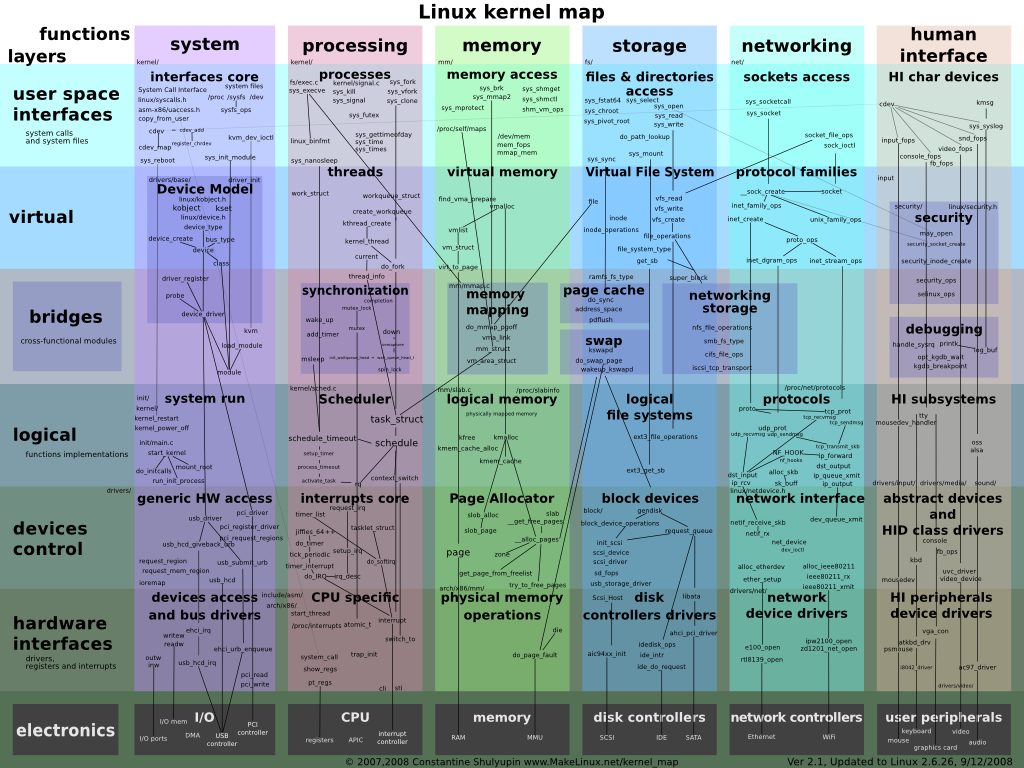
\includegraphics[width=23cm]{pictures/linux_map}
\caption{Carte du noyau Linux 2.6}
\label{fig:linuxmap}
\end{figure}
\end{landscape}

\end{appendices}

\backmatter

%\printglossary

% bibliography
%\nocite{*}
%\bibliography{bibliography}
%\bibliographystyle{plain}

\printindex

\end{document}
